\chapter[Analysis]{Analysis}\label{chap:analysis}

This chapter constitutes the core of this dissertation. Here, we will discuss the analysis conducted, starting with a general overview, followed by an explanation of the samples, triggers, and object definitions. We will then talk about the corrections applied to the data and simulations to enhance the analysis results. Additionally, we will cover the criteria used in event selection and how the signal and background have been modeled. Finally, we will present the expected upper limits of the branching ratio for each channel, as this analysis will only be working with simulated signal, alongside simulated and real background data. The chapter concludes by addressing the subsequent steps required before data unblinding and the attainment of the final experimental measurement, as well as suggesting other ideas to improve the results.

\section{Analysis overview}\label{sec:analysis_overview}

This analysis uses data from proton-proton collisions corresponding to an integrated luminosity of 39.54 fb$^{-1}$ at $\sqrt{s}=$13 TeV, collected by the CMS detector at LHC in 2018 during Run 2. It only targets the Higgs boson production mode via gluon fusion (ggH), which accounts for approximately 87\% of the Higgs boson production at LHC at $\sqrt{s}=$13 TeV. Although it is possible to extend this analysis to include more production modes, time constraints have led us to focus to the main production channel. The final states of interest consist of an isolated and energetic photon, a charged meson pair, and photons compatible with a third (and sometimes fourth) neutral meson, with 0 hadronic jets and no additional leptons ($e/\mu$). The mesons considered here are a $\phi$, a $\omega$ and a $D^{*0}$, each further decaying into two charged particles and a third (and fourth) neutral one (see Table \ref{tab:Higgs_rare_decays_three}).

\begin{table}[ht]
    \centering
    \begin{tabular}{ll}
        $\text{H}\decaysto \phi\gamma$ ,& $\phi\decaysto \pi^+\pi^-\pi^0$ \\
        $\text{H}\decaysto \omega\gamma$ ,& $\omega\decaysto \pi^+\pi^-\pi^0$\\
        $\text{H}\decaysto D^{*0}\gamma$ ,& $D^{*0}\decaysto D^{0}\pi^{0}/\gamma,\ D^{0}\decaysto K^{\mp}\pi^{\pm}$\\
        $\text{H}\decaysto D^{*0}\gamma$ ,& $D^{*0}\decaysto D^{0}\pi^{0}/\gamma,\ D^{0}\decaysto K^{\mp}\pi^{\pm}\pi^{0}$
    \end{tabular}
    \caption{Higgs rare decays under study in this analysis.}
    \label{tab:Higgs_rare_decays_three}
\end{table}

The analysis strategy involves categorizing events to increase the signal to background ratio. In our production mode (ggH), the largest background source in this analysis consists of $\gamma$ plus jets events.

The branching fractions of rare Higgs boson decays to a meson and photon can be computed using a factorization approach in QCD. The calculation considers both direct and indirect contributions, as explained in the first chapter and depicted in Figure \ref{fig:Higgs_rare_decay_veritces}. The interference between these components is significant. In the SM, the indirect component dominates, and the Higgs boson couplings to light quarks are probed by searching for modifications in this branching fraction due to interference effects.

As previously explained, given the exotic nature of the decays under study, the theoretical decay widths being so small, the large hadronic background at the LHC, and the limited amount of data collected, we cannot aim for precise measurements of the branching fractions. Instead, the end goal of this thesis is to calculate a reasonable upper limit on the branching ratio of the aforementioned Higgs boson decays, using Monte Carlo (MC) samples to model the SM expected signal. To obtain a competitive, real result, this initial estimation requires further refinement and improvement, such as considering additional background sources, systematic uncertainties, etc.

The main difference between this analysis and the study of the three decays in the upper half of Table \ref{tab:Higgs_rare_decays} is that, in contrast to those, we are studying 3-body decays with neutral particles, which are more challenging to track than charged ones. The framework used for this analysis builds upon the existing framework for the simpler two-body decays currently under analysis by the Particle Physics Collaboration at the Massachusetts Institute of Technology (MIT). To extend their study to include three-body decays involving neutral particles, our main focus has been on accurately recovering the missing neutral particles.

\section{Samples and triggers}\label{sec:samples_triggers}

To develop this analysis, the data file format used is one designed by CMS, which is an extended version of \verb+NANOAOD+. It is based on the official \verb+NANOAODv9+ recipe and includes the reconstructed mesons, as described in Section \ref{sec:objects}, as additional objects. The \verb+NANOAOD+ format consists of an Ntuple-like structure used by CMS, which can be read using bare root, and containing the per-event information that is needed in most generic analyses \cite{CMS:NanoAOD}. This analysis is performed using the \verb+ROOT+ data analysis framework, an open-source data analysis tool commonly used in high energy physics written mainly in C++ \cite{CERN:root}.

\subsection{Data and Tau trigger}\label{subsec:data_tau_trigger}

Events are selected from proton-proton collision data at a center-of-mass energy of $\sqrt{s}=$13 TeV and a bunch spacing of 25 ns, collected by the CMS experiment during the LHC's Run 2 in 2018, corresponding to a total integrated luminosity of 39.54 fb$^{-1}$. Good run ranges and luminosity blocks are chosen based on criteria encoded in a golden JSON file.

To filter data in the gluon fusion production mode, a tau-like trigger is employed. This Tau trigger selects a photon with $\pT^{\gamma} > 35\ \GeV$ and a ditrack system with $\pT^{\text{jet}} > 35\ \GeV$, after going through the L1 trigger, which also imposes rapidity restrictions of $\abs{\eta^{\gamma}}<2.1$ and $\abs{\eta^{\text{jet}}}<2.1$. The trigger is applied to both data and MC. Introduced in 2018, this trigger recorded events enriched in gluon fusion production of the Higgs boson and VBF that were not registered by the dedicated trigger, providing an effective luminosity of 39.54 fb$^{-1}$. The trigger selecting events during 2018 is encoded as \verb+Photon35_TwoProngs35+. \todo{Should I include trigger efficiencies for each channel in the appendix? If so, how do I obtain these plots?} The datasets used in gluon fusion and VBF analysis are detailed in Table \ref{tab:ggH_datasets}.

\begin{table}[ht]
    \centering
    \begin{tabular}{|c|c|c|}
        \hline
        \multicolumn{1}{|c|}{\cellcolor{lightgray}Year} & \cellcolor{lightgray}Dataset & \cellcolor{lightgray}Integrated luminosity [fb$^{-1}$] \\ \hline
        2018    & \verb+/Tau/Run2018B-UL2018+  & 0.67 \\
        2018    & \verb+/Tau/Run2018C-UL2018+  & 6.94 \\
        2018    & \verb+/Tau/Run2018D-UL2018+  & 31.93 \\ \hline
    \end{tabular}
    \caption{Datasets used in the gluon fusion analysis from the campaign MiniAODv2 of the MINIAOD data tier.}
    \label{tab:ggH_datasets}
\end{table}

\subsection{Background simulation}

The background estimation will ultimately rely solely on data. However, at the early stage of this analysis, simulated samples are used to understand the background processes affecting the different selected final states. The main background process for the gluon fusion production mode is a single photon and jets.

Every event is generated at leading order (LO) precision using the MADGRAPH5 generator \verb+MG5_aMC@NLO+ \cite{Alwall:2014hca} and POWHEG \cite{Alioli:2010xd}, while PYTHIA8 \cite{Sjostrand:2014zea} is used for the hadronization. For all simulations, the NNPDF 3.1 \cite{NNPDF:2017mvq} next-to-next-to-leading-order (NNLO) parton distribution functions (PDFs) are used, while the modeling of the underlying event is generated using the CMS Pythia 5 (CP5) tunes \cite{CMS:2019csb}. The Run 2 legacy reconstruction algorithms \cite{Elmetenawee:2020emw} are used for all the MC and data samples. The campaign and global tag used to produce the background and signal MC samples are \verb+RunIISummer20UL18MiniAODv2-106X+ and \verb+upgrade2018_realistic_v16_L1v1+, respectively. Table \ref{tab:MC_samples} summarizes the list of datasets used for the study along with their cross sections \cite{CERN:xsdb}.

\begin{table}[ht]
    \centering
    \begin{tabular}{|l|c|}
        \hline
        \multicolumn{1}{|c|}{\cellcolor{lightgray}Monte Carlo name} & \cellcolor{lightgray}Cross section [pb] \\ \hline
        \verb+GJets_HT-40To100_TuneCP5_13TeV-madgraphMLM-pythia8+  & 18540 (LO) $\times$ 1.26 \\
        \verb+GJets_HT-100To200_TuneCP5_13TeV-madgraphMLM-pythia8+  & 8644 (LO) $\times$ 1.26 \\
        \verb+GJets_HT-200To400_TuneCP5_13TeV-madgraphMLM-pythia8+  & 2183 (LO) $\times$ 1.26 \\
        \verb+GJets_HT-400To600_TuneCP5_13TeV-madgraphMLM-pythia8+  & 260.2 (LO) $\times$ 1.26 \\
        \verb+GJets_HT-600ToInf_TuneCP5_13TeV-madgraphMLM-pythia8+  & 86.58 (LO) $\times$ 1.26 \\ \hline
    \end{tabular}
    \caption{MC samples used for the gluon fusion production mode. The normalization of $\gamma+$jets is scaled by 1.26 \cite{CMS:2018qao} \todo{WHY?}.}
    \label{tab:MC_samples}
\end{table}

\subsection{Signal simulation}

The only Higgs boson production mode studied, gluon fusion, is generated at next-to-leading order (NLO) using the POWHEGv2 event generator extended with the MiNLO procedure \cite{Hamilton:2012np}. The production rates and kinematic distributions for the Higgs boson with $m_H=125\ \GeV$ are assumed throughout. In particular, the cross section for gluon fusion is computed at NNLO in QCD and NLO in electroweak accuracy, resulting in 48.58 pb, as provided by the LHC Higgs Cross Section Working Group in Ref. \cite{LHCHiggsCrossSectionWorkingGroup:2016ypw}.

The decay of the Higgs boson is handled by Pythia, and it does not simulate direct and indirect effective vertices. The expected SM branching fractions of the Higgs rare decays are as previously shown in Table \ref{tab:Higgs_rare_decays_values}: $\mathcal{B}(\text{H}\decaysto \phi\gamma) = (2.31 \pm 0.11)\times 10^{-6}$ and $\mathcal{B}(\text{H}\decaysto \omega\gamma) = (1.48 \pm 0.08)\times 10^{-6}$, while $\mathcal{B}(\text{H}\decaysto D^{*0}\gamma)$ has not yet been computed. In the analysis, however, the branching ratios are set to
\begin{equation*}
    \mathcal{B}(\text{H}\decaysto \phi\gamma) = \mathcal{B}(\text{H}\decaysto \omega\gamma) = \mathcal{B}(\text{H}\decaysto D^{*0}\gamma) = 1\ .
\end{equation*}
This is because then, when computing a limit, the obtained value is directly the measured upper limit of the branching ratio itself. If we were to set the branching fractions to the SM values, the measured quantities would be the signal strengths, i.e., the factors by which the observed fractions exceed the SM values. The branching fractions of the meson decays used are also shown in Table \ref{tab:Higgs_rare_decays}, but further detailed in Table \ref{tab:Meson_decay_br}.

\begin{table}[!ht]
    \centering
    \begin{tabular}{|l|c|}
        \hline
        \multicolumn{1}{|c|}{\cellcolor{lightgray}Meson decay channel} & \multicolumn{1}{c|}{\cellcolor{lightgray} SM $\mathcal{B}$ (\%)} \\ \hline
        $\phi\decaysto \pi^+\pi^-\pi^0$     & $15.4 \pm 0.4$   \\
        $\omega\decaysto \pi^+\pi^-\pi^0$   & $89.2 \pm 0.7$   \\
        $D^{*0}\decaysto D^{0}\pi^0$        & $64.7 \pm 0.9$   \\
        $D^{*0}\decaysto D^{0}\gamma$       & $35.3 \pm 0.9$   \\
        $D^{0}\decaysto K^{\mp}\pi^{\pm}$           & $3.962 \pm 0.031$   \\
        $D^{0}\decaysto K^{\mp}\pi^{\pm}\pi^0$      & $14.43 \pm 0.50$   \\
        \hline
    \end{tabular}
    \caption{Meson decay branching ratios used throughout the analysis, from the PDG \cite{PDG}.}
    \label{tab:Meson_decay_br}
\end{table}

\section{Object definitions}\label{sec:objects}

This analysis primarily relies on photons and charged tracks to extract the final state signature of exclusive hadronic decays, while also making use of other physics objects such as additional leptons (or the lack thereof) and hadronic jets to suppress background. All used objects, except the mesons, are discussed in this section, with the next section dedicated solely to meson reconstruction.
\vspace*{-6pt}
\begin{myitemlist}
    \item[Primary vertex (PV):] To consider an event, it must contain at least one primary vertex, which is regarded as the vertex of the hard interaction. There should be a minimum of four tracks associated with the selected primary vertex (from the Higgs boson, the photon and the ditrack system). For events with multiple selected vertices, the PV is chosen to be the vertex corresponding to the hardest scattering in the event, determined using tracking information alone, as described in Ref. \cite{Contardo:2015bmq}.

    \item[Jets:] During the reconstruction of a proton-proton (pp) collision, jets are often reconstructed with a $\pT$ that differs from that of the final-state particles within the jet. The jet energy corrections (JEC) adjust the reconstructed jet energy to match the true energy of the final-state particles. The CMS collaboration has developed a factorized approach to these JEC, consisting of multiple levels that correct various physics or detector effects. This approach provides flexibility in the corrections to suit various types of analyses. These correction levels are commonly referred to as L1FastJet, L2Relative, L3Absolute, and L2L3Residual.

    The flow of these JEC is as follows: jets are reconstructed from particle flow (PF) candidates using the anti-$k_\text{T}$ clustering algorithm with a distance parameter of $R = 0.4$ as implemented by FastJet \cite{Cacciari:2011ma}. Jets within this small cone (referred to as AK4 jets for $R = 0.4$) are selected among those with $\pT > 20\ \GeV$ and $\abs{\eta} < 4.7$ for forward tagging. At the LHC, a significant number of pp collisions occur simultaniously during one bunch crossing, with soft ones contaminating the collision of interest. To mitigate this effect, known as \textit{pileup} (PU), charged hadrons not originating from the primary vertex are removed using the charged hadron subtraction (CHS) algorithm \cite{CMS:2014ata, Perloff:2012wpa}. The tight pileup ID criterion is applied to reduce the contamination of jets with $\pT < 50\ \GeV$ initiated by the pileup interactions. Jets are corrected for the response inside the detector, differentially in $\abs{\eta} - \abs{\phi}$, for the pileup contributions, and for data only, the residual difference observed between data and simulation.
    
    In the current analysis version, the \verb+Summer19UL+ jet energy corrections set is used, as well as the DeepJet tagging algorithm with the medium working point to identify $b$-jets \cite{Bols:2020bkb}.

    \item[Missing energy:] The $\pT^{\text{miss}}$ measures the transverse momentum imbalance in the event. To estimate it, the deepMET algorithm \cite{Feng:2744871} is used, and $\pT^{\text{miss}}$ filters are then applied to account for instrumental noise in the detector and minimize the impact of the non-collisional background.
    
    \item[Photons:] Photon candidates are reconstructed as SuperCluster objects in the ECAL with $\ET > 38\ \GeV$ and $\abs{\eta^{\gamma}} < 2.1$ in both the barrel and endcap regions. In addition, photons have to satisfy the multivariate analysis (MVA) based selection identification (mvaID) criteria following the \verb+Fall17IsoV2+ recipe \cite{CMS:2020uim}. For the production mode used, the mvaID provides 80\% (90\%) signal selection efficiency for the endcap (barrel) region. The mvaID criteria include photon isolation, charged hadron isolation, and require photons to pass shower shape preselection cuts \cite{Rembser:2019ijh}. The photon's ECAL cluster must be inconsistent with charged particle tracks reconstructed in the silicon tracker to reject electrons faking photons, achieved using a conversion safe electron veto. Residual $\ET$ -dependent photon energy scale and smearing corrections are applied. Additional photons with looser requirements ($\ET > 20\ \GeV$ and the WP90 version of the photonID) are also vetoed to reduce the potential contribution of diphotons. Table \ref{tab:photon_selection} summarizes the criteria for photon selection.

    \begin{table}[!ht]
        \centering
        \begin{tabular}{|l|c|}
            \hline
                \multicolumn{2}{|c|}{\cellcolor{lightgray}Selection criteria ($\gamma$ from PV)}\\ \hline
                $\pT^{\gamma}$            &$>38$ GeV\\
                $\abs{\eta^{\gamma}}$       &$<2.1$ \\
                mvaID                       &WP90/WP80 \\
                electron Veto               &Yes \\\hline
            \end{tabular}
        \caption{Selection criteria applied to the photon from the primary vertex.}
        \label{tab:photon_selection}
    \end{table}

    An additional correction was attempted, involving shifting the photon's origin to that of the PV of the meson. This slight adjustment to the initial coordinates led to a minor change in the four-momentum variables of the photon, but it did not consistently reduce the discrepancy with the generation-level particle values. Consequently, it was discarded and not used.

\end{myitemlist}

\section{Meson reconstruction \todo{ADD FOURTH D0* CHANNEL}}\label{sec:meson_reconstruction}

The $\phi$, $\omega$ and $D^{*0}$ mesons decay products are reconstructed using charged particle tracks measured in the tracker, as well as energy deposited in the ECAL compatible with neutral particles coming also from the PV. For the $\phi$ and $\omega$ mesons, the targeted charged ditrack is $\pi^\pm\pi^\mp$, while for the $D^{*0}$ meson the charged ditrack is $K^{\mp}\pi^{\pm}$.

In the following sections, the term \textit{ditrack system} will refer to the system of the two charged tracks, and even though they not form a real particle, notions like ditrack mass will be used (understand the mass of the ditrack as the mass component of the sum of the four-momenta of both tracks). To refer to the meson originating from the PV, namely $\phi$, $\omega$ and $D^{*0}$, terms like \textit{meson} or \textit{full meson} will be used, emphasizing that the neutral particles have been accounted for. Some considerations have been made to precisely reconstruct the full meson:
\vspace*{-6pt}
\begin{myitemlist}
    \item[Track selection:] To be selected, the tracks need to satisfy a ``high purity'' reconstruction criteria, which considers the number of tracker layers with hits, track fit quality, and the impact parameter values relative to their uncertainties. For a detailed description of the algorithm, refer to Ref. \cite{CMS:2014pgm}.

    \item[Meson decay vertex:] The meson decay vertex is determined using the standard CMSSW \cite{CMSSW} kinematic vertex fitting package, as described in Ref. \cite{Prokofiev:2005zz}. Using the candidate's decay vertex and its associated momentum, a newly fitted transient track is constructed to represent the meson candidate. Then, for each primary vertex, the track is extrapolated to the nearest point in 3D space. The meson vertex's longitudinal distance is required to be within 24 cm from the center of the detector.
    
    \item[Isolation:] To ensure good track selection, a dedicated isolation criterion of the candidate based on the tracks is used. This dimensionless isolation parameter (Iso) is determined from the meson's momentum and other tracks within a cone of radius $\Delta R = 0.3$ around the ditrack system's direction. Only tracks with $\pT > 0.9\ \GeV$ associated with the same meson vertex are considered, excluding the charged-hadron candidates that define the ditrack. The definition is as follows:
    \begin{equation*}
        \text{Iso} = \frac{\pT^{\text{meson}}}{\pT^{\text{meson}}+\sum_{\text{trk}}{\abs{\pT^{\text{trk}}}}}
    \end{equation*}
    A high isolation value will be required to consider a meson candidate (over 0.9).

    \item[Neutral particle photons:] For each selected ditrack, up to two photons with $\pT > 5 \ \GeV$ are recovered in a small cone of $\Delta R = 0.05$ around the ditrack direction. These photons account for the recovery of neutral particles, as $\pi^{0}\decaysto\gamma\gamma$ in $\sim 98.8\%$ with $c\tau=25$ nm \cite{PDG}. From generation-level MC we know that photons coming from neutral particle decays that in turn come from the three-body decays must be very collimated with the ditrack system. In the case of the $\phi$/$\omega$ channels and the $D^{*0}$ channel when $D^{0}$ decays into three bodies, these photons directly originate from the $\pi^0$ of the three-body decay. In the case of the $D^{*0}$ channel, the photon comes either directly from $D^{*0}\decaysto D^{0}\gamma$ or from de decay of the $\pi^0$ from $D^{*0}\decaysto D^{0}\pi^0$.
    
    \item[Ditrack mass hypothesis:] The invariant mass of the refitted ditrack system is also used to reduce contamination from background events. The mass of the pair, assuming the charged-pion hypothesis for the two tracks, is consistent with the charged components of the $\phi$ and $\omega$ mesons. Since the ditrack system is not a real resonance, its mass is very wide but consistent and useful for reducing background events. In the case of the $D^{*0}$ channel, two scenarios are considered. On the one hand, when $D^{0}$ decays into a pair of charged particles (kaon-pion) the ditrack system's invariant mass is a real narrow resonance (namely $D^{0}$) coherent with the mass of that meson. On the other hand, when $D^{0}$ decays into a pair of charged particles and a neutral pion, one finds the same scenario as for the $\phi$/$\omega$ decay channels.
    
    The exact used selection criteria will be presented at the end of this section, but it is worth noting that for the $\phi$/$\omega$ three-body decays involving a $\pi^0$, the mass of the ditrack is approximately two-thirds of the full meson's mass (each pion carries roughly a third of the energy).

    Furthermore, instead of recovering the ditrack invariant mass by only retrieving the mass component of the sum of both four-momenta, the CMSSW kinematic fit has been employed. To study the performance of this fit, it is useful to define the \textit{residual} as the difference between the reconstructed values and the corresponding generation-level ones. Figure \ref{fig:kinematic_fit_residuals} displays the residual of the ditrack invariant mass reconstruction with and without the kinematic fits with vertex constraint for every decay mode.
    \begin{figure}[!ht]
        \captionsetup[subfigure]{labelformat=empty}
        \vspace*{-0.2cm}
        \centering
        \setlength{\mylength}{\textwidth}
        \begin{subfigure}[t]{0.50\mylength}
                \centering
                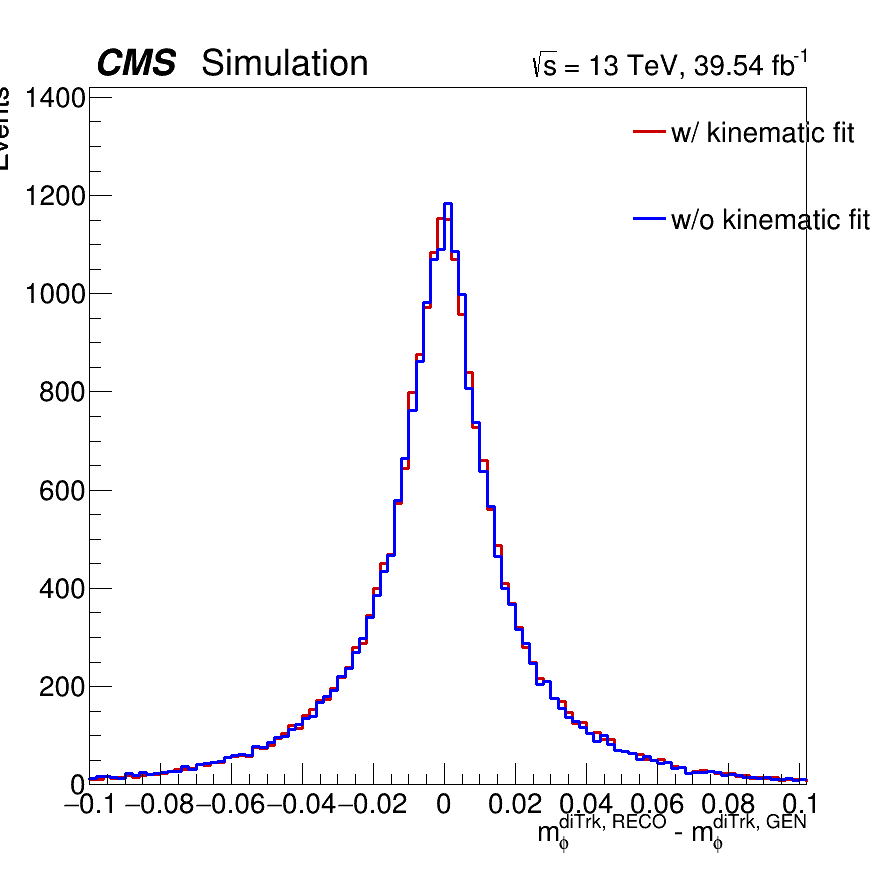
\includegraphics[width=0.45\mylength]{resources/plots/Phi3_kinematic_fit_residual.png}
                \caption{\footnotesize (a)}
        \end{subfigure}%
        \begin{subfigure}[t]{0.50\mylength}
                \centering
                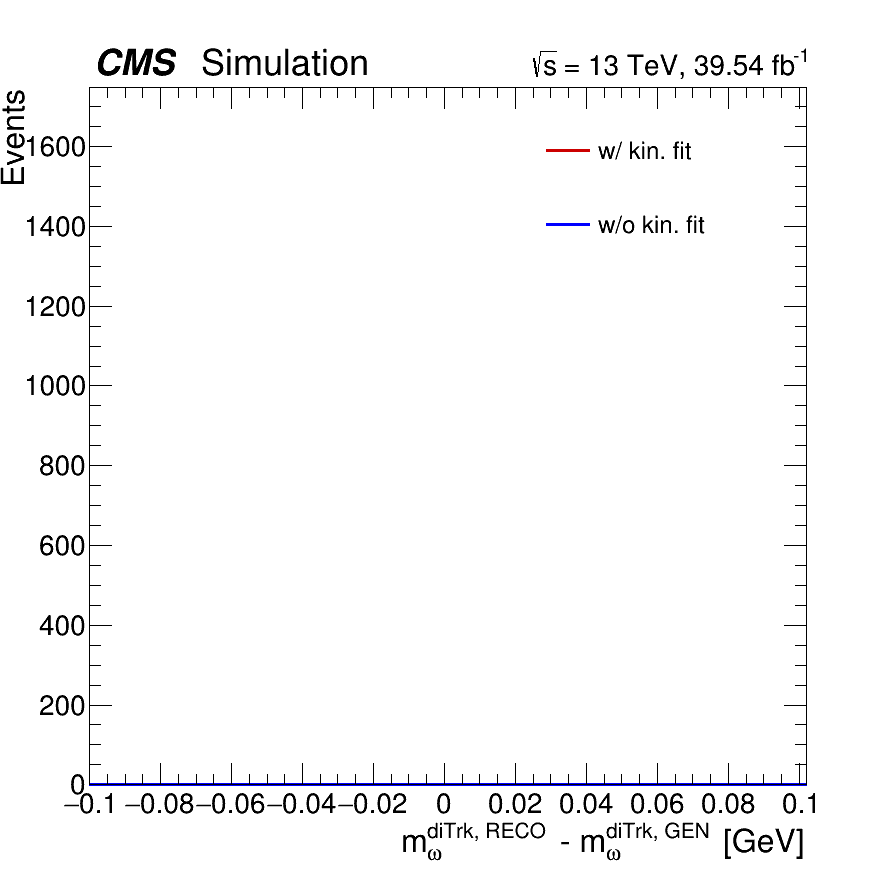
\includegraphics[width=0.45\mylength]{resources/plots/Omega_kinematic_fit_residual.png}
                \caption{\footnotesize (b)}
        \end{subfigure}%\begin{subfigure}[t]{0.50\mylength}\baselineskip
        \vskip\baselineskip
        \vspace*{-0.1cm}
        \begin{subfigure}[t]{0.50\mylength}
                \centering
                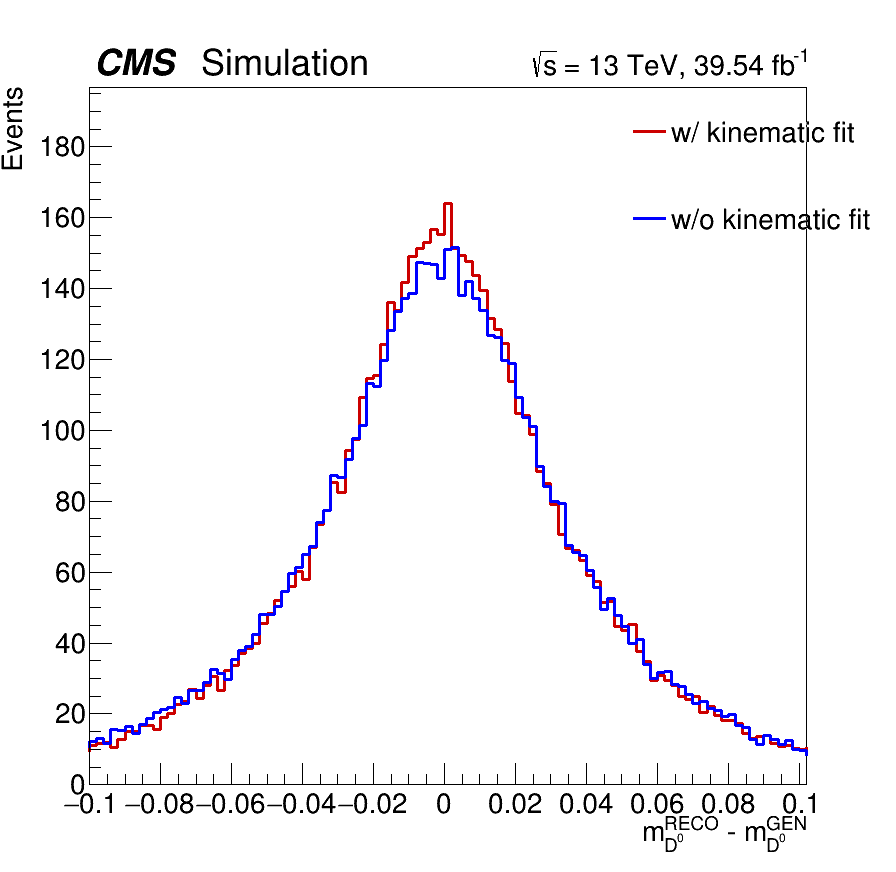
\includegraphics[width=0.45\mylength]{resources/plots/D0Star_2body_kinematic_fit_residual.png}
                \caption{\footnotesize (c)}
        \end{subfigure}%\begin{subfigure}[t]{0.50\mylength}
        \begin{subfigure}[t]{0.50\mylength}
                \centering
                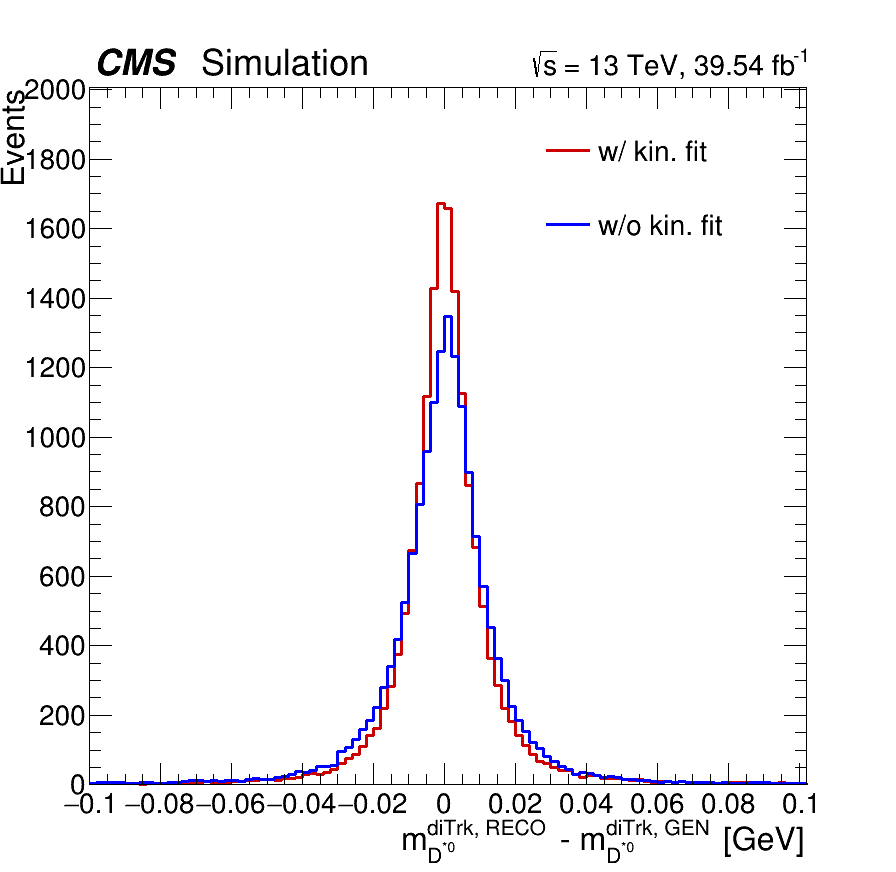
\includegraphics[width=0.45\mylength]{resources/plots/D0Star_3body_kinematic_fit_residual.png}
                \caption{\footnotesize (d)}
        \end{subfigure}%
        \vspace*{-0.0cm}
        \caption{Ditrack mass residuals for the different decay channels. (a) is for $\phi$, (b) is for $\omega$, (c) is for $D^{*0}$ 2-body, and (d) is for $D^{*0}$ 3-body.}
        \label{fig:kinematic_fit_residuals}
        \vspace*{-0.0cm}
    \end{figure}
    Table \ref{tab:kinematic_fit_RMSE} shows the root mean squared errors with respect to generation-level, both with and without the kinematic fit, for each channel. Applying the kinematic fit improves the reconstructed ditrack invariant mass values for all channels.

    \begin{table}[!ht]
        \centering
        \begin{tabular}{|l|c|C{2.9cm}@{}c|}
            \hline
            \cellcolor{lightgray}Decay channel & \cellcolor{lightgray}RMSE without kinematic fit & \multicolumn{2}{c|}{\cellcolor{lightgray}RMSE with kinematic fit} \\ \hline
            $\phi$          &37.8 MeV   &34.0 MeV  & (-10\%)   \\
            \r$\omega$        &\r xx.x MeV   & x\r x.x MeV &\r (-x\%)  \\
            $D^{*0}$ 2-body &49.7 MeV   &47.6 MeV  & (-4\%)     \\
            $D^{*0}$ 3-body &73.3 MeV   &55.5 MeV  & (-24\%)    \\
            \hline
            \end{tabular}
        \caption{Root mean squared errors (RMSE) with and without the kinematic fit for each decay mode.}
        \label{tab:kinematic_fit_RMSE}
    \end{table}
    
    \item[Meson mass hypothesis:] The simplest way to reconstruct the four-momentum of the full meson is by summing the four-momenta of the ditrack system and those from the photons compatible with the decay of neutral particles. This approach was initially used for all channels. Nevertheless, for the $\phi$, $\omega$ and $D^{*0}$ 3-body decay channels, additional corrections were applied.
    
    Consider that the photons in the $\Delta R$ cone come from the $\pi^{0}\decaysto\gamma\gamma$ decay. When only one photon is recovered, it means that either both photons ended up in the same ECAL crystal, or that one of them was too soft to be measured ($\pT < 5\ \GeV$) and therefore only one is detected. Following the first hypothesis, we can interpret the energy deposited in the same ECAL cell as the energy from the full pion. To account for this, whenever only one photon is recovered, we assign this object a non-zero mass (the pion's mass) before adding the four-momenta. This correction is of very low energy, and thus the changes in $\pT$, $\eta$ or $\phi$ of the full meson are imperceptible, but its mass is visibly affected. Figure \ref{fig:full_meson_mass_residuals} and Table \ref{tab:full_meson_mass_residuals_RMSE} show the residual of the full meson invariant mass reconstruction and the RMSE, respectively, with and without the $\pi^0$ mass correction for the $\phi$ and $\omega$ decay modes.
    \begin{figure}[!ht]
        \captionsetup[subfigure]{labelformat=empty}
        \vspace*{-0.2cm}
        \centering
        \setlength{\mylength}{\textwidth}
        \begin{subfigure}[t]{0.50\mylength}
                \centering
                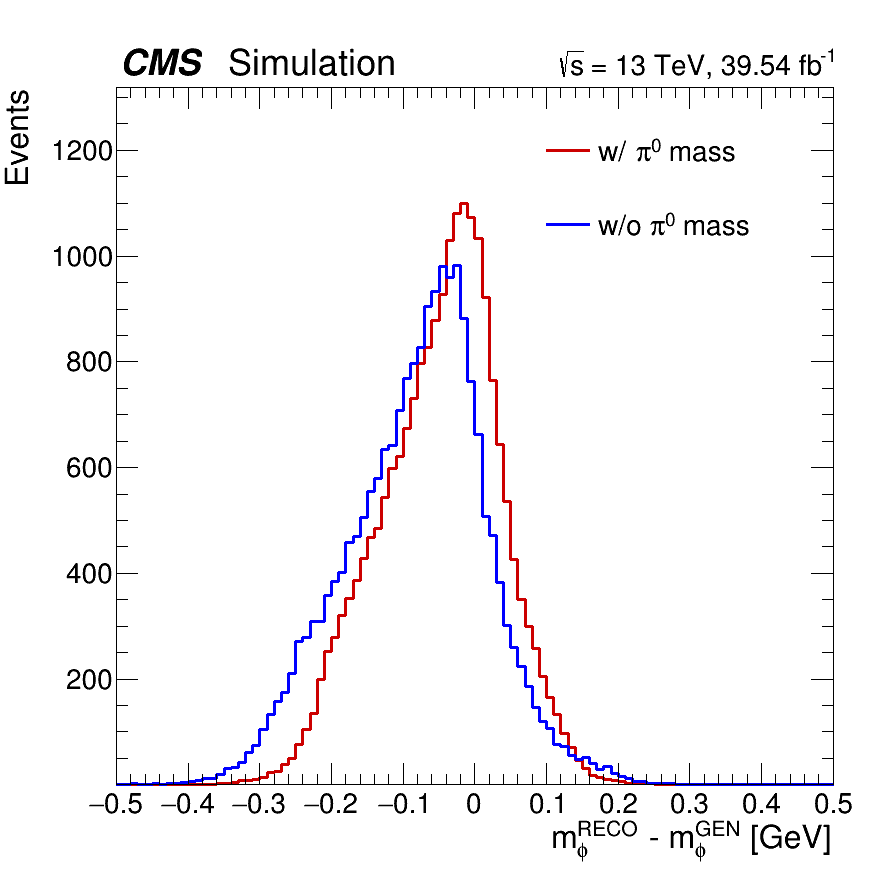
\includegraphics[width=0.45\mylength]{resources/plots/Phi3_fullmeson_mass_residual.png}
                \caption{\footnotesize (a)}
        \end{subfigure}%
        \begin{subfigure}[t]{0.50\mylength}
                \centering
                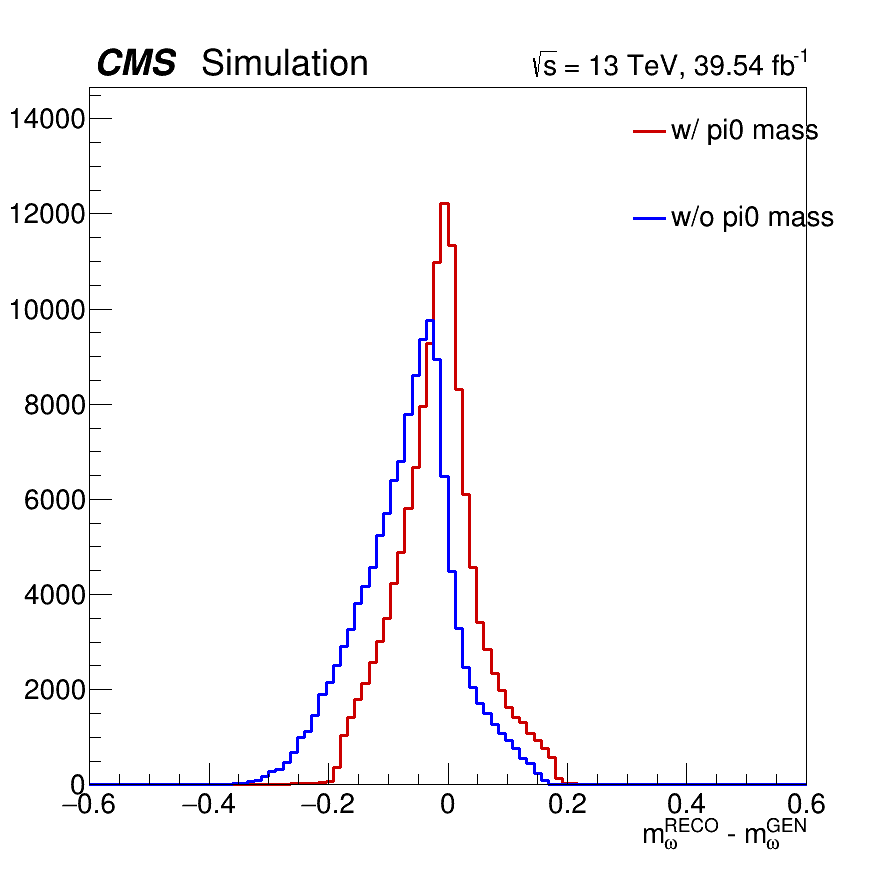
\includegraphics[width=0.45\mylength]{resources/plots/Omega_fullmeson_mass_residual.png}
                \caption{\footnotesize (b)}
        \end{subfigure}%\begin{subfigure}[t]{0.50\mylength}\baselineski
        \caption{Full meson mass residuals for the different decay channels. (a) is for $\phi$, (b) is for $\omega$.}
        \label{fig:full_meson_mass_residuals}
        \vspace*{-0.0cm}
    \end{figure}

    This slight improvement will enable us to narrow some selection cuts and reduce more background events, ultimately improving the final result.

    \begin{table}[!ht]
        \centering
        \begin{tabular}{|l|c|C{3.2cm}@{}c|}
            \hline
            \cellcolor{lightgray}Decay channel & \cellcolor{lightgray}RMSE without $m_{\pi^0}$ correction& \multicolumn{2}{c|}{\cellcolor{lightgray}RMSE with $m_{\pi^0}$ correction} \\ \hline
            $\phi$          &130.2 MeV   &117.7 MeV  & (-10\%)   \\
            $\omega$        &127.9 MeV   &113.1 MeV  & (-12\%)   \\
            \hline
            \end{tabular}
        \caption{Root mean squared errors with and without the $m_{\pi^0}$ correction for the $\phi$ and $\omega$ decay modes.}
        \label{tab:full_meson_mass_residuals_RMSE}
    \end{table}

    An additional correction was attempted. The idea was to reconstruct the neutral particle by summing the recovered photons, and then forcing the reconstructed neutral particle to have the $\pi^0$'s mass while maintaining the energy and direction ($\eta$ and $\phi$) unchanged. This required a slight modification of the neutral particle's transverse momenta, as given by
    \begin{equation*}
        \pT = \sqrt{(E^2 - m^2)(1-\tanh^2\eta)}\ .
    \end{equation*}
    When adding this neutral particle to the ditrack, the full meson's $\pT$ remained effectively unchanged, and the full meson's mass was very similar (and slightly worse) compared to using the previous technique. Therefore, this adjustment was not used.

    \item[Meson transverse momentum correction:] To compute the upper limits of the branching ratios of the decays, the Higgs boson invariant mass is going to be calculated. To achieve an accurate value, it is crucial to recover the two involved objects, namely the photon and the full meson, with the utmost precision. There are seven variables in play: the components of the four-momenta, four of which belong to the meson and three to the photon. The accuracy of the Higgs boson's invariant mass relies mainly on the accuracy of the transverse momenta of both particles involved. The other five variables ($\eta$ and $\phi$ of both particles and the mass of the full meson) are either already well measured or, in the case of the mass, too low in energy to significantly impact the computation. Improving the transverse momentum of the photon is very challenging, as it already undergoes the reconstruction algorithm briefly discussed in the previous section. Thus, the main emphasis should be on recovering the $\pT$ of the full meson as precisely as possible.
    
    \begin{figure}[!ht]
        \captionsetup[subfigure]{labelformat=empty}
        \vspace*{-0.2cm}
        \centering
        \setlength{\mylength}{\textwidth}
        \begin{subfigure}[t]{0.50\mylength}
                \centering
                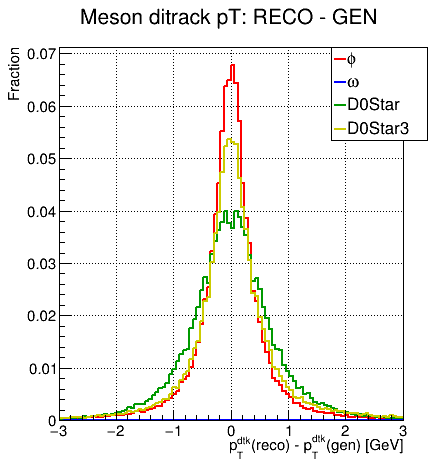
\includegraphics[width=0.45\mylength]{resources/plots/ditrack_residuals_pt.png}
                \caption{\footnotesize (a)}
        \end{subfigure}%
        \begin{subfigure}[t]{0.50\mylength}
                \centering
                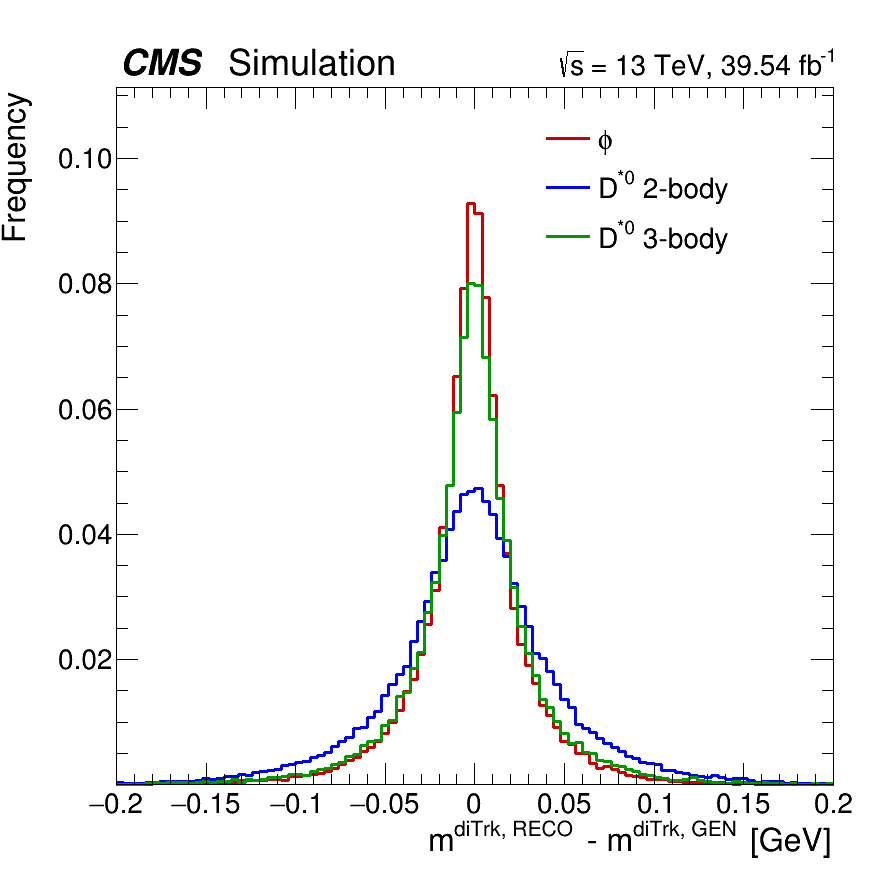
\includegraphics[width=0.45\mylength]{resources/plots/ditrack_residuals_mass.png}
                \caption{\footnotesize (b)}
        \end{subfigure}%\begin{subfigure}[t]{0.50\mylength}\baselineskip
        \vskip\baselineskip
        \vspace*{-0.1cm}
        \begin{subfigure}[t]{0.50\mylength}
                \centering
                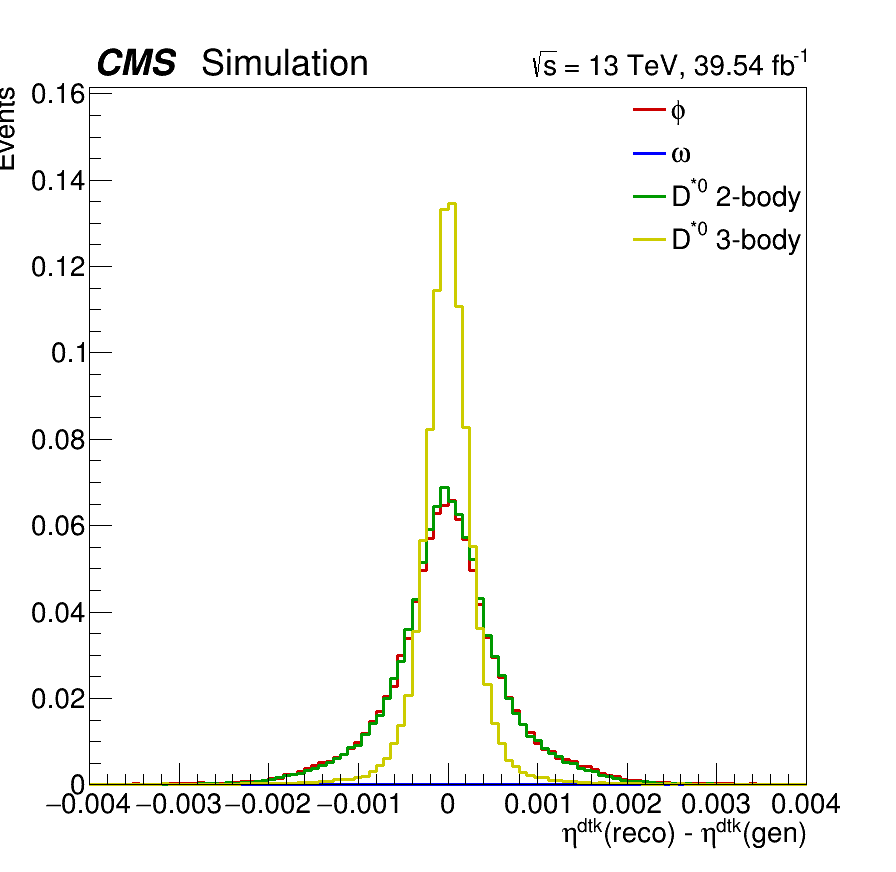
\includegraphics[width=0.45\mylength]{resources/plots/ditrack_residuals_eta.png}
                \caption{\footnotesize (c)}
        \end{subfigure}%\begin{subfigure}[t]{0.50\mylength}
        \begin{subfigure}[t]{0.50\mylength}
                \centering
                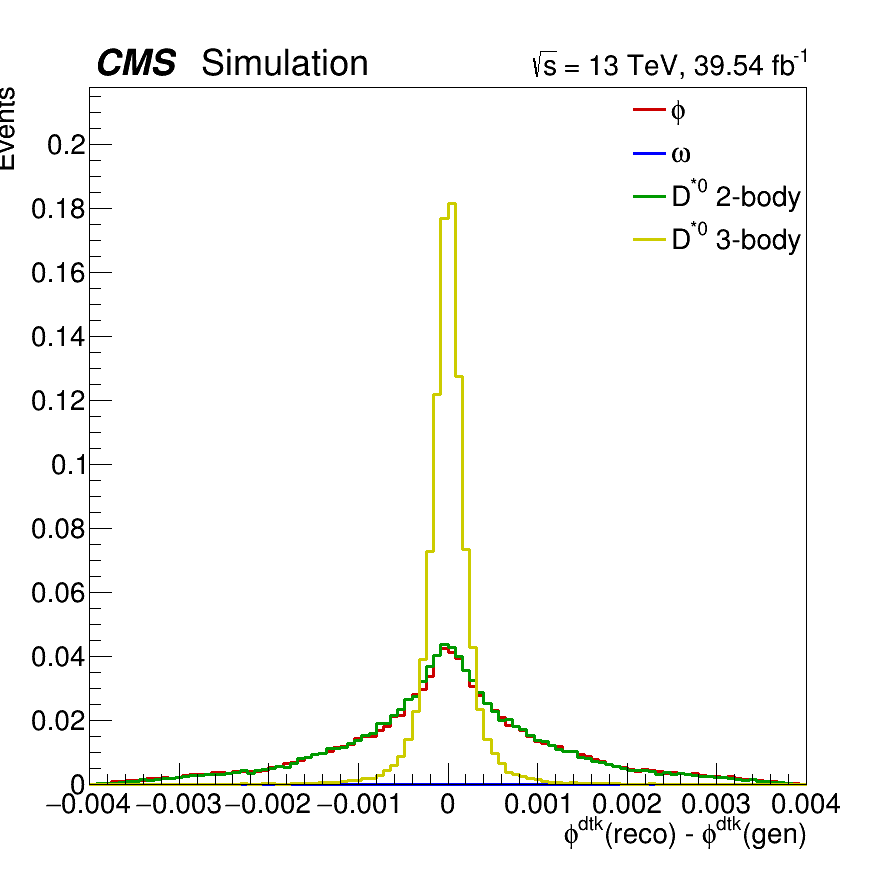
\includegraphics[width=0.45\mylength]{resources/plots/ditrack_residuals_phi.png}
                \caption{\footnotesize (d)}
        \end{subfigure}%
        \vspace*{-0.0cm}
        \caption{Ditrack residuals for the different four-momentum components of each decay channel. (a) is for $\pT$, (b) is for the mass, (c) is for $\eta$, and (d) is for $\phi$.}
        \label{fig:ditrack_residuals}
        \vspace*{-0.0cm}
    \end{figure}
    In each decay channel, the ditrack system variables are measured with remarkable accuracy. Figure \ref{fig:ditrack_residuals} displays the residuals of the ditrack transverse momentum, mass, $\eta$ and $\phi$ with respect to their generation-level MC value for every decay mode. All histograms are normalized to the same area for comparing the various channels. It is worth noting that, as the ditrack consists of a pair of charged tracks that can be precisely determined thanks to the silicon tracker, the direction -- $\eta$ and $\phi$ -- is accurately measured for all channels.

    The initial approach to reconstruct the full meson's transverse momentum is to sum the four-momenta of the ditrack system and those from the photons compatible with the decay of neutral particles. The main source of discrepancy between the full meson's transverse momenta and their generation-level MC values arises from the poorly reconstructed neutral particles. Given that the pions decay into softer photons that are hard to recover, many events exhibit missing energy, resulting in the full meson's $\pT$ being generally less energetic than expected. Figure \ref{fig:fullmeson_residuals_pt} shows the residuals of the full meson's transverse momentum with respect to their generation-level MC value for each decay mode.
    \begin{figure}[!ht]
        \captionsetup[subfigure]{labelformat=empty}
        \vspace*{-0.2cm}
        \centering
        \setlength{\mylength}{\textwidth}
        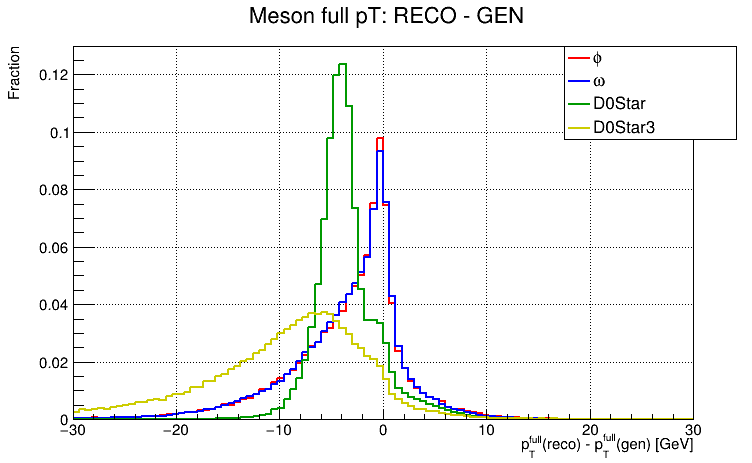
\includegraphics[width=0.75\mylength]{resources/plots/fullmeson_residuals_pt.png}
        \caption{Transverse momentum residuals for the full meson for each decay channel.}
        \label{fig:fullmeson_residuals_pt}
        \vspace*{-0.0cm}
    \end{figure}
    Both the $\phi$ and $\omega$ channels exhibit an asymmetric left shoulder, consistent with the hypothesis of missing energy from the neutral particle. The $D^{*0}$ 2-body, on the other hand, is more symmetric but displaced about 5 GeV, since the soft $\pi^{0}/\gamma$ from $D^{*0}\decaysto D^{0}\pi^{0}/\gamma$ typically carries around $\sim5$ GeV in energy. The right shoulder results from events in which we can recover one photon compatible with this missing neutral particle, which is only around $\sim 13\%$ of events. The $D^{*0}$ 3-body combines characteristics from all previous channels, and since it is missing two neutral particles it is noticeably shifted towards the lower end of the axis.

    To address this issue, dedicated Boosted Decision Trees (BDTs) have been implemented for each channel using the Toolkit for Multivariate Data Analysis for \verb+ROOT+ \cite{CERN:root}, also known as \verb+TMVA+ \cite{TMVA:2007ngy}. This machine learning (ML) technique will correct for the full meson's $\pT$. A boosted decision tree (BDT) is a ML binary classifier or regressor algorithm based on a flowchart-like structure in which each internal node represents a test on an attribute, each branch signifies the test's outcome, and each leaf node denotes a class level. For more detailed information, refer to Refs. \cite{TMVA:2007ngy, Coadou:2022nsh}.

    The variables used in all models are presented in Table \ref{tab:model_variables}.
    \begin{table}[!ht]
        \centering
        \begin{tabular}{|c|c|c|}
            \hline
            \multicolumn{3}{|c|}{\cellcolor{lightgray} Regression input variables} \\ \hline
            \cellcolor{lightgray}Dimensionless  &\cellcolor{lightgray}Dimensionful  &\cellcolor{lightgray}Normalised            \\\hline
            $\eta^{\text{diTrk}}$                           &$\pT^{\gamma_1}$       &$\pT^{\text{meson}}/\pT^{\gamma}$          \\
            $\Delta R^{\gamma_1, \text{diTrk}}$             &$\pT^{\gamma_2}$       &$\pT^{\text{meson}}/\pT^{\text{diTrk}}$    \\
            $\Delta R^{\gamma_2, \text{diTrk}}$             &$m^{\text{diTrk}}$     &           \\
            $\Delta R^{\text{diTrk}}$                       &$m^{\text{meson}}$ ($^*$)  &       \\
            $\Delta(\eta^{\gamma}, \eta^{\text{diTrk}})$    & & \\
            $\Delta(\phi^{\gamma}, \phi^{\text{diTrk}})$    & & \\
            \hline
        \end{tabular}
        \caption{Input variables for the BDTs. $\gamma_1$ and $\gamma_2$ represent photons from neutral particle decay, $\gamma$ stands for the Higgs boson decay photon. The asterisk denotes exclusion for $D^{*0}$ 2/3-body decay.}
        \label{tab:model_variables}
    \end{table}
    The variables labeled by $\gamma_1$ and $\gamma_2$ refer to the recovered photons compatible with the decay of the neutral particles, while $\gamma$ refers to the photon originating in the Higgs boson decay. The dimensionless variables $\Delta R^{\gamma_1, \text{diTrk}}$ and $\Delta R^{\gamma_2, \text{diTrk}}$ reference the angular separation between each photon and the ditrack system. $\Delta R^{\text{diTrk}}$ is the angular separation within the track pair. It is worth defining $\Delta(\eta^{\gamma}, \eta^{\text{diTrk}})$ and $\Delta(\phi^{\gamma}, \phi^{\text{diTrk}})$,
    \begin{equation*}
        \begin{aligned}
        \Delta(\eta^{\gamma}, \eta^{\text{diTrk}}) &= \eta^{\text{diTrk}} - \eta^{\gamma} \\
        \Delta(\phi^{\gamma}, \phi^{\text{diTrk}}) &= (\phi^{\text{diTrk}} - \phi^{\gamma}) \modu 2\pi \in[0, 2\pi)\ .
        \end{aligned}
    \end{equation*}
    The $\Delta(\phi^{\gamma}, \phi^{\text{diTrk}})$ definition has this form because the angular variable $\phi$ is periodic. The asterisk ($^*$) next to the full meson's mass indicates that this variable is not included for the $D^{*0}$ 2-body or 3-body decay, as in these channels, $m^{\text{meson}}$ is not very precisely determined.

    The variables in Table \ref{tab:model_variables} have been thoughtfully selected after many model iterations, ensuring low correlation between them and with the Higgs boson invariant mass, while maintaining reasonable predictive power.

    All the models have been trained to predict not the correct value of the full meson's transverse momentum, but a scale factor $\pT^{\text{meson, GEN}}/\pT^{\text{meson, RECO}}$ instead. This scale factor represents the adjustment needed for the reconstructed $\pT$ to match its generation-level MC value. The motivation for this approach is to avoid biasing the model by predicting a dimensionless variable.

    We implemented the BDTs using the \verb+TMVA+ framework, specifically the
\begin{small}
\vspace*{-6pt}
\begin{verbatim}
TMVA::Factory.BookMethod(dataloader, TMVA::Types::kBDT, "modelName", "<options>");
\end{verbatim}
\vspace*{-6pt}
\end{small}
    method, with the ML regressor \verb+TMVA::Types::kBDT+. To prevent overtraining, we employed cross-validation by rotating the training and testing samples. Specifically, the signal MC was divided into three subsets: A, B, and C. Three models with identical hyperparameters were trained on A+B (B+C / C+A) and tested on C (A / B). This approach ensures all the available data is used to train the models while testing them on signal MC that was not used for training. To recover all the signal events, these three models were then applied to their respective testing subsets. Afterward, all the subsets were combined once more, resulting in a complete set of events.

    \begin{figure}[!ht]
        \captionsetup[subfigure]{labelformat=empty}
        \vspace*{-0.2cm}
        \centering
        \setlength{\mylength}{\textwidth}
        \begin{subfigure}[t]{0.50\mylength}
            \centering
            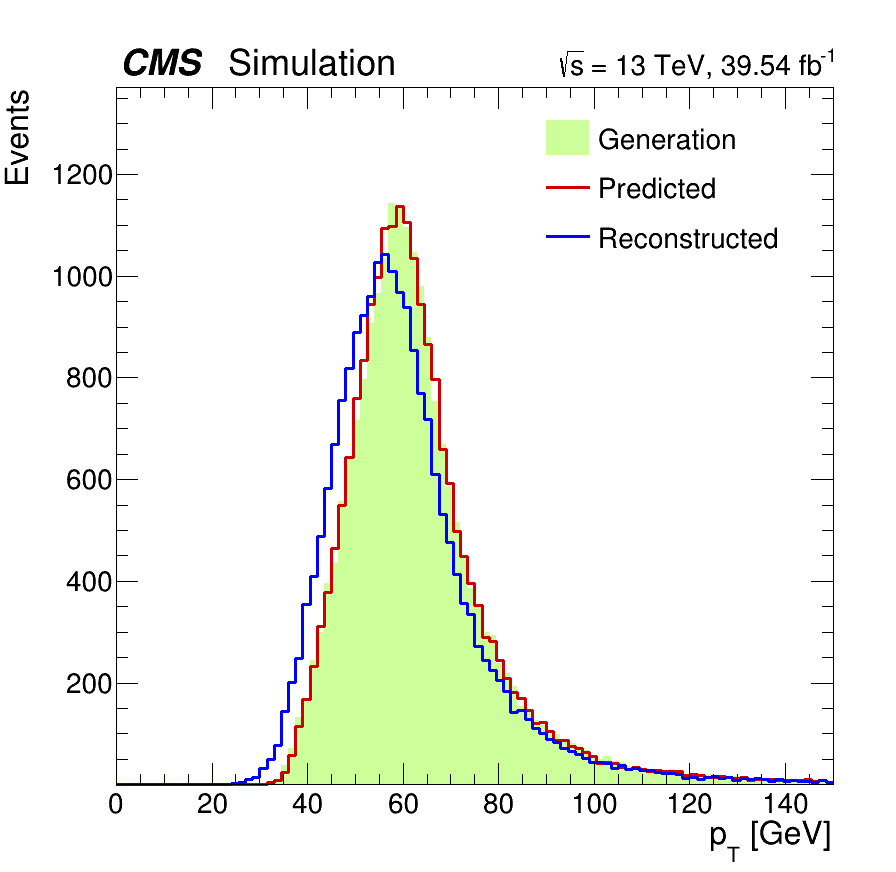
\includegraphics[width=0.45\mylength]{resources/plots/Phi3_model_pt.png}
            \caption{\footnotesize (a)}
        \end{subfigure}%
        \begin{subfigure}[t]{0.50\mylength}
            \centering
            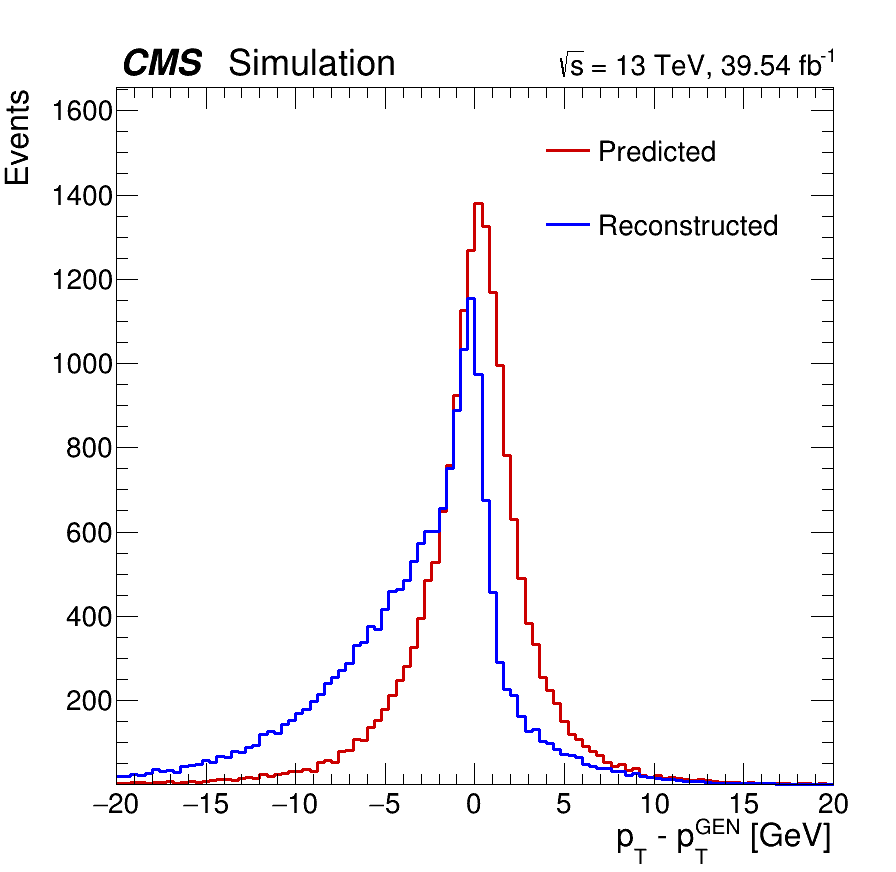
\includegraphics[width=0.45\mylength]{resources/plots/Phi3_model_pt_residuals.png}
            \caption{\footnotesize (b)}
        \end{subfigure}%\begin{subfigure}[t]{0.50\mylength}\baselineskip
        \vskip\baselineskip
        \vspace*{-0.1cm}
        \begin{subfigure}[t]{0.50\mylength}
            \centering
            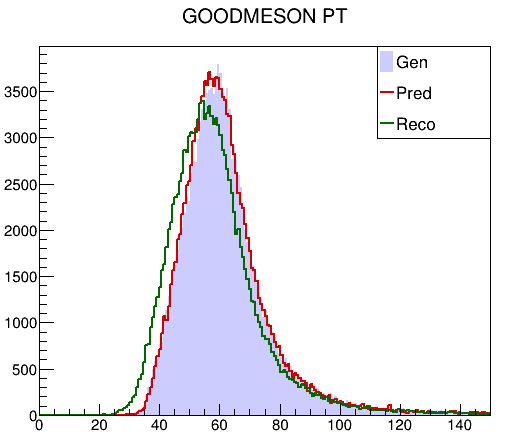
\includegraphics[width=0.45\mylength]{resources/plots/Omega_model_pt.png}
            \caption{\footnotesize (c)}
        \end{subfigure}%
        \begin{subfigure}[t]{0.50\mylength}
            \centering
            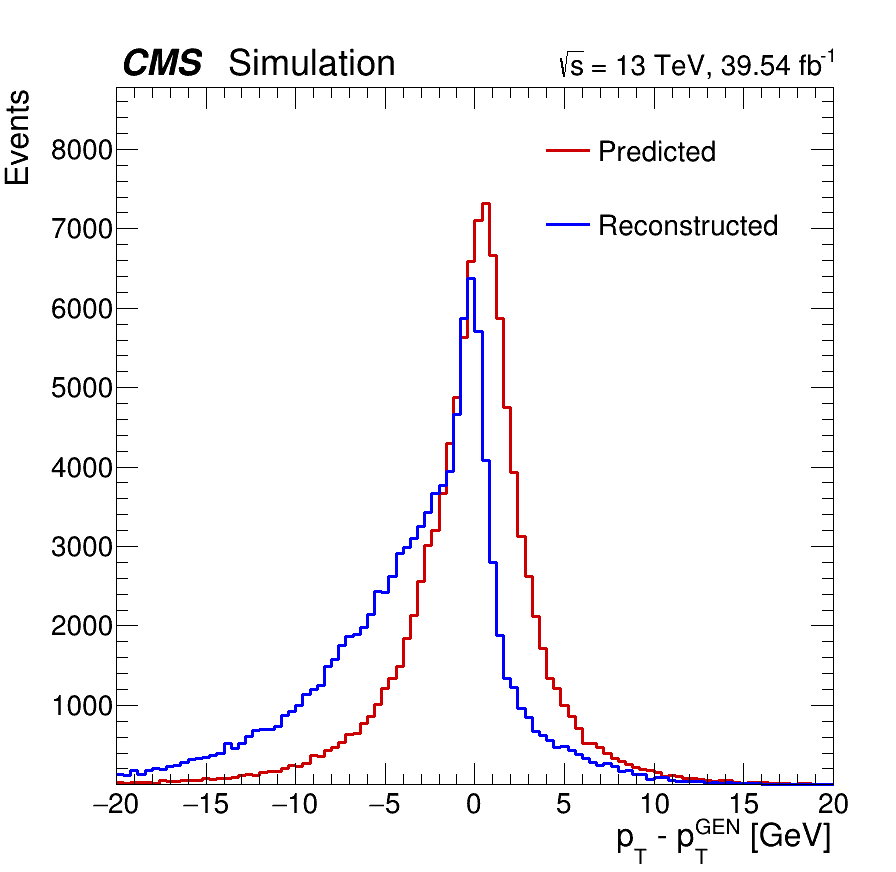
\includegraphics[width=0.45\mylength]{resources/plots/Omega_model_pt_residuals.png}
            \caption{\footnotesize (d)}
        \end{subfigure}%\begin{subfigure}[t]{0.50\mylength}\baselineskip
    \caption{Transverse momentum of the $\phi$ and $\omega$ mesons. (a/c) Display the generation-level MC transverse momenta in blue, the prediction by the BDT in red, and the recovery by the initial approach in green, for the $\phi/\omega$ mesons, respectively. (b/d) Show the residuals with (red) and without (green) the BDT prediction, for the $\phi/\omega$ mesons, respectively.}
    \label{fig:pt_residuals_model_omega_phi}
        \vspace*{-0.0cm}
    \end{figure}
    The hyperparameters for each model are available in Table \ref{tab:hyperparameters_models} in Appendix \ref{sec:appendix_models}. Figures \ref{fig:pt_residuals_model_omega_phi} and \ref{fig:pt_residuals_model_d0star} compare the generation-level MC transverse momentum with the reconstruction values, both with and without regression, and show the residuals for each channel.
    \begin{figure}[!ht]
        \captionsetup[subfigure]{labelformat=empty}
        \vspace*{-0.2cm}
        \centering
        \setlength{\mylength}{\textwidth}
        \begin{subfigure}[t]{0.50\mylength}
            \centering
            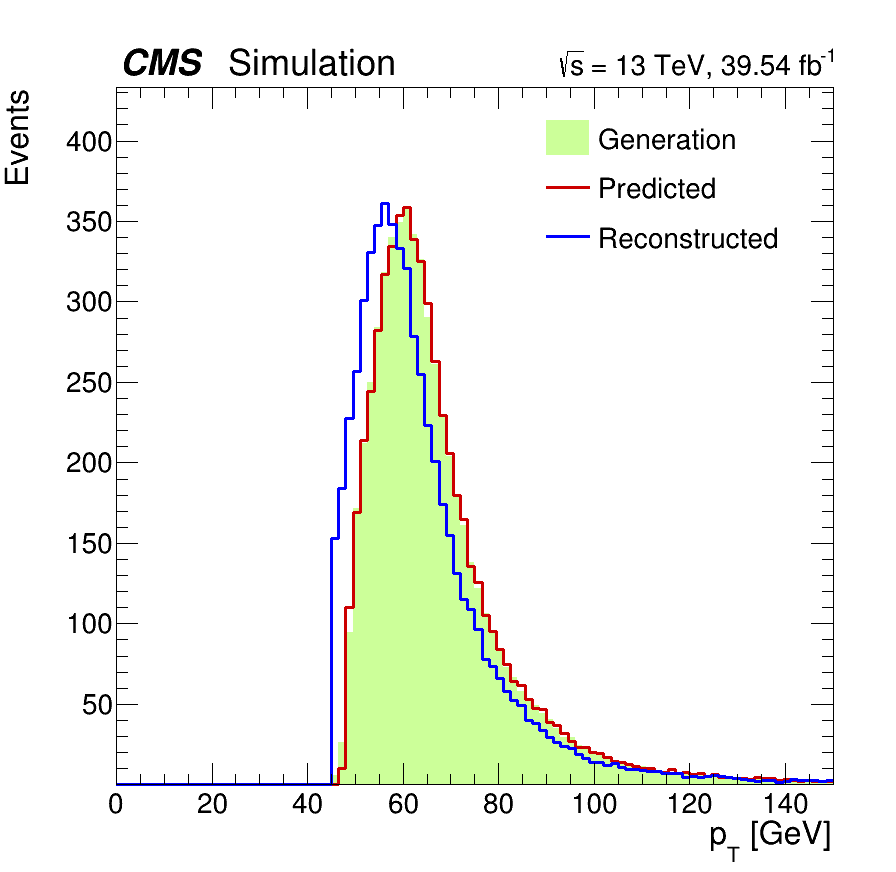
\includegraphics[width=0.45\mylength]{resources/plots/D0Star_2body_model_pt.png}
            \caption{\footnotesize (a)}
        \end{subfigure}%
        \begin{subfigure}[t]{0.50\mylength}
            \centering
            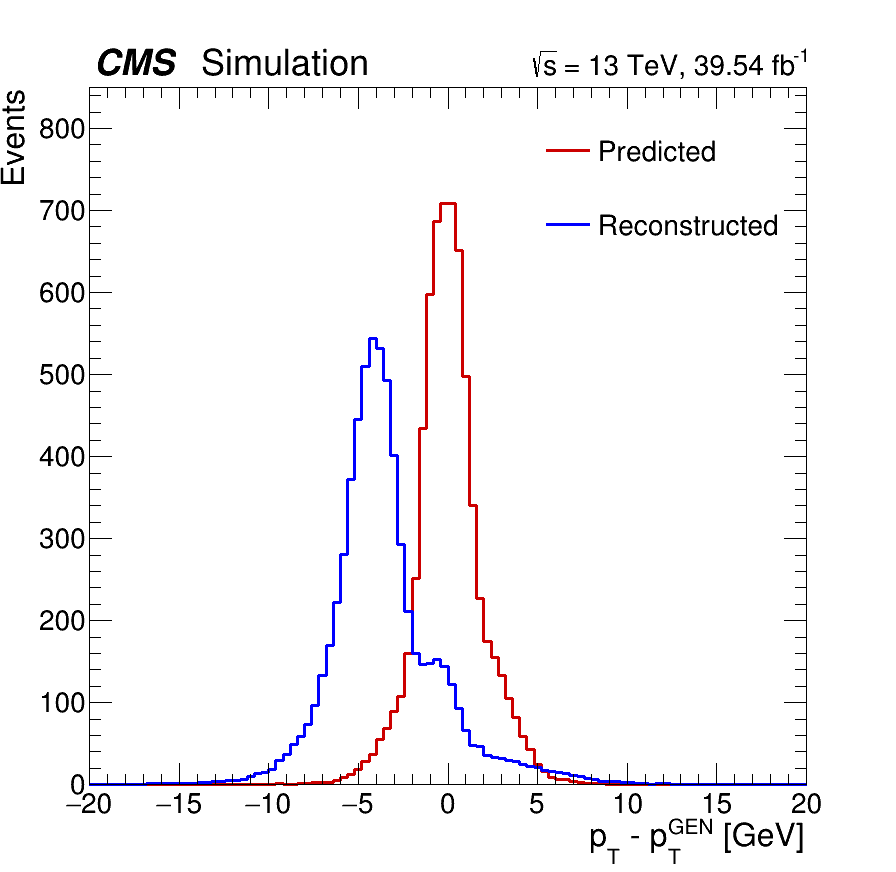
\includegraphics[width=0.45\mylength]{resources/plots/D0Star_2body_model_pt_residuals.png}
            \caption{\footnotesize (b)}
        \end{subfigure}%\begin{subfigure}[t]{0.50\mylength}\baselineskip
        \vskip\baselineskip
        \vspace*{-0.1cm}
        \begin{subfigure}[t]{0.50\mylength}
            \centering
            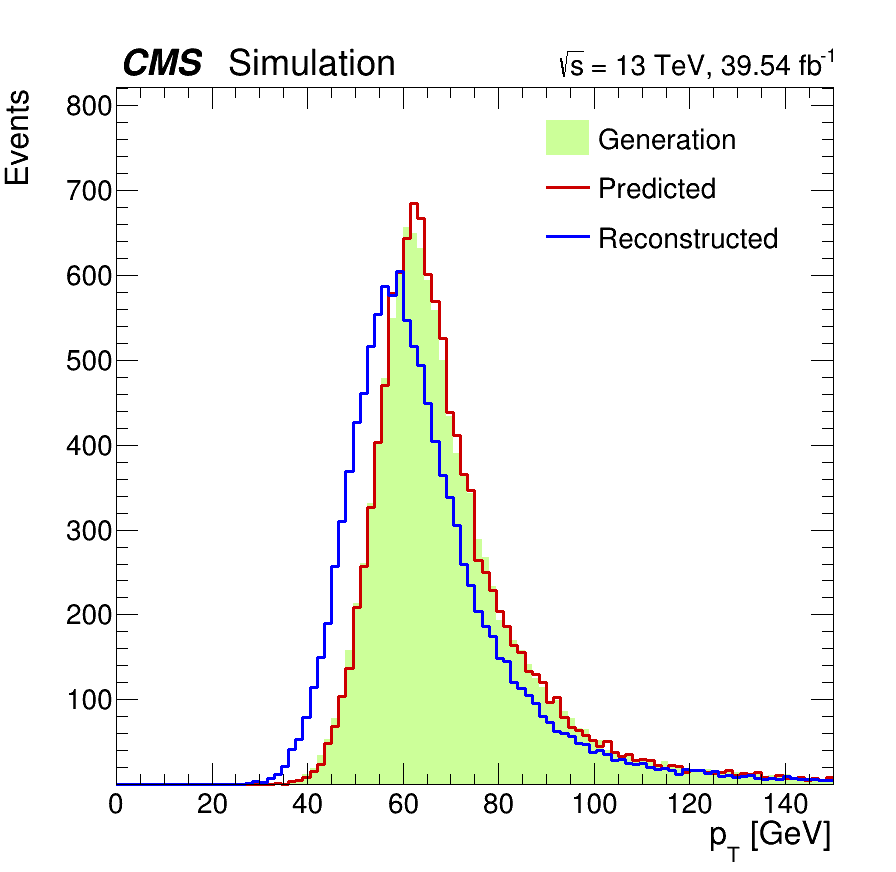
\includegraphics[width=0.45\mylength]{resources/plots/D0Star_3body_model_pt.png}
            \caption{\footnotesize (c)}
        \end{subfigure}%
        \begin{subfigure}[t]{0.50\mylength}
            \centering
            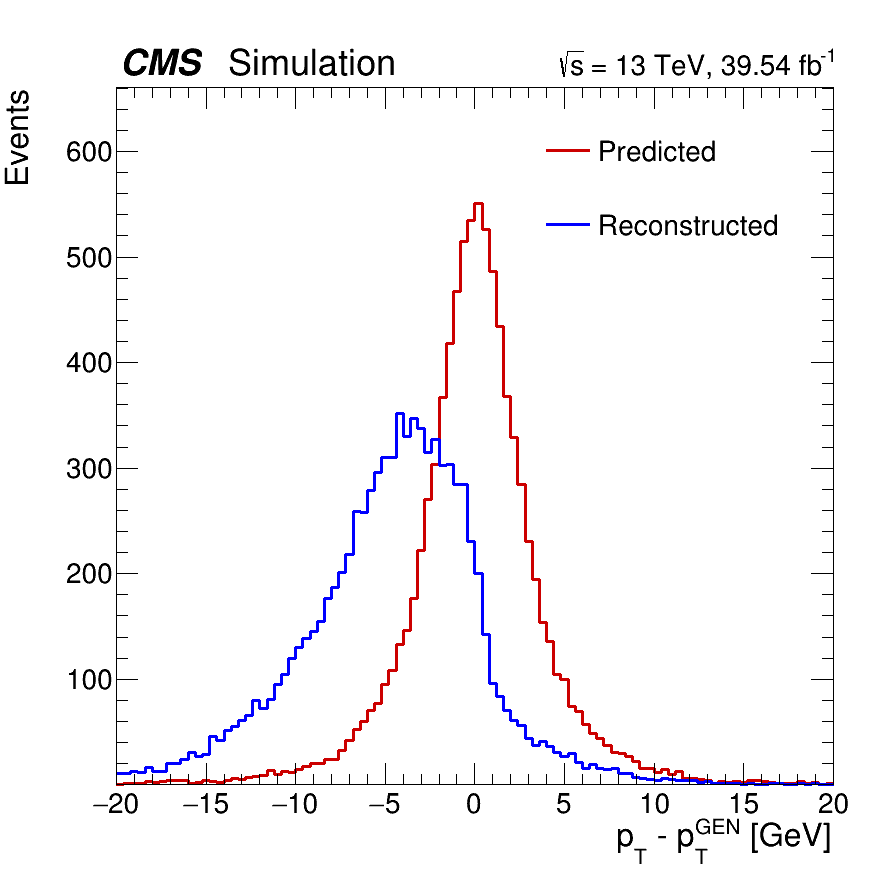
\includegraphics[width=0.45\mylength]{resources/plots/D0Star_3body_model_pt_residuals.png}
            \caption{\footnotesize (d)}
        \end{subfigure}%\begin{subfigure}[t]{0.50\mylength}\baselineskip
    \caption{Transverse momentum of the $D^{*0}$ meson in both the 2-body and 3-body decay channels. (a/c) Display the generation-level MC transverse momenta in blue, the prediction by the BDT in red, and the recovery by the initial approach in green, for the 2/3-body decay channel, respectively. (b/d) Show the residuals with (red) and without (green) the BDT prediction, for the 2/3-body decay channel, respectively.}
    \label{fig:pt_residuals_model_d0star}
        \vspace*{-0.0cm}
    \end{figure}

    Both channels displayed in Figure \ref{fig:pt_residuals_model_omega_phi} are quite similar. For both full mesons, the predicted transverse momentum spectrum aligns well with the generation-level one. Additionally, the residuals for the predicted values are centered around the origin and symmetric, indicating that the predicted $\pT$ no longer exhibits missing energy. The 2-body decay channel presented in Figure \ref{fig:pt_residuals_model_d0star} shows that the model accurately shifts by around 5 GeV, as the residuals are narrow around 0 GeV instead of around -5 GeV, and it is also more symmetric than the initially reconstructed $\pT$. \todo{The 3-body decay channel shown in Figure \ref{fig:pt_residuals_model_d0star} bla bla bla}.

    Table \ref{tab:models_pt_RMSE} shows the root mean squared errors with respect to generation-level transverse momentum, both with and without the BDT regression, for each channel. Applying the transverse momenta regression noticeably improves the value and reduces the error for all channels by around 35\%.
    \begin{table}[!ht]
        \centering
        \begin{tabular}{|l|c|C{3.1cm}@{}c|}
            \hline
            \cellcolor{lightgray}Decay channel & \cellcolor{lightgray}RMSE without $\pT$ regression & \multicolumn{2}{c|}{\cellcolor{lightgray}RMSE with $\pT$ regression} \\ \hline
            $\phi$          &5.124 GeV   &3.480 GeV  & (-32\%)  \\
            $\omega$        &5.058 GeV   &3.339 GeV  & (-34\%)  \\
            $D^{*0}$ 2-body &3.132 GeV   &1.871 GeV  & (-40\%)  \\
            \r$D^{*0}$ 3-body &\r xx.x GeV   &x\r x.x GeV  & \r(-xx\%)  \\
            \hline
            \end{tabular}
        \caption{Root mean squared errors of the full meson's transverse momentum with and without the BDT regression for each decay mode.}
        \label{tab:models_pt_RMSE}
    \end{table}
    The applied BDTs not only significantly reduce the error in the transverse momentum of the full meson for every channel but also restore the symmetric residual shape of the variable. This indicates that the estimated $pT$ values are as likely to be underestimated as to be overestimated, accounting for the missing energy from the undetected neutral particles. This reduction in the width of the residuals will directly lead to an improved, lower upper limit on the Higgs boson branching fraction.

    A crucial consideration in developing any ML model is overtraining, and this case is no exception. This is the primary reason a dimensionless scale factor was predicted rather than the direct value of the momentum. In our situation, overtraining can be directly detected by examining the background shape after applying the regression. If the model learns that, regardless of the input, the predicted value should lead to a peak around 125 GeV when constructing the Higgs invariant mass variable, we know it is overtrained and biased and needs to be rejected. To address this and reject biased models, we introduced a \textit{background shaping function (BSF)} that provides a dimensionless metric which increases as the model becomes more biased. The BSF we developed for measuring each model is defined to be
    \begin{equation*}
        BSF \propto -A\log{(\mu-125)^2} + B N + C \sqrt{b}\ ,
    \end{equation*}
    where $A$, $B$, and $C$ are constants, $\mu$ is the peak of a fitted double-sided Crystal Ball\footnote{A double-sided Crystal Ball function, named after the Crystal Ball Collaboration \cite{A2:CB}, is a probability density function (PDF) commonly used in high-energy physics (HEP). It is built from a Gaussian center and two asymmetric tails modeled by power-law functions. Additional details about this PDF and its implementation in ROOT can be found in Ref. \cite{CERN:root_CB}.} (CB) to the Higgs boson's invariant mass constructed from background MC events, $N$ is the normalization constant of the Crystal Ball, and $b$ is the number of events in the interval $(117, 133)$ GeV of the Higgs boson's invariant mass. Note that the BSF depends only on background events, especially in reconstructing the Higgs boson's invariant mass. The first factor penalizes the model more when the background Higgs boson's invariant mass shape peaks around $m_H=125\ \GeV$, because the background should be flat or asymptotically falling near that value. The remaining two factors account for the number of events near the expected signal peak. More background events result in a smaller and thus worse signal-to-background ratio, a quantity we want to maximize to improve the computation of upper limits.

    Figure \ref{fig:BSF_vs_RMSE_phi} shows the BSF as a function of the RMSE of different models applied to reconstruct the transverse momentum of the $\phi$ meson.
    \begin{figure}[!ht]
        \captionsetup[subfigure]{labelformat=empty}
        \vspace*{-0.2cm}
        \centering
        \setlength{\mylength}{\textwidth}
        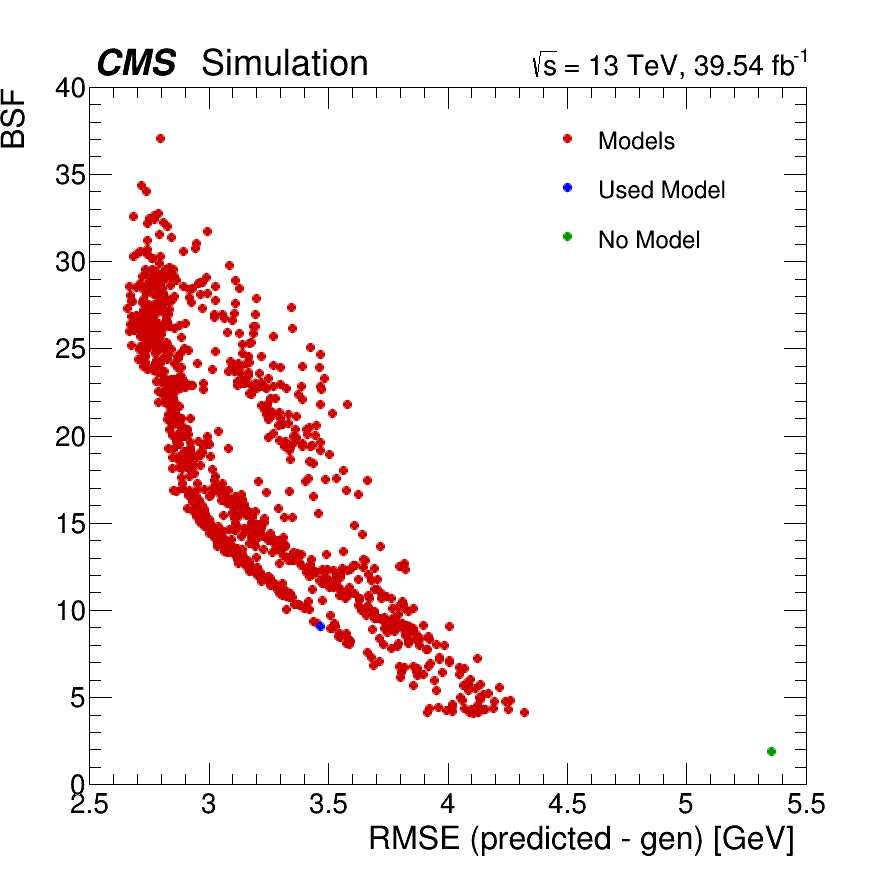
\includegraphics[width=0.85\mylength]{resources/plots/BSF_vs_RMSE_phi.png}
        \caption{Background shaping function (BSF) as a function of the root mean squared error (RMSE) of the $\pT$ for various models of the $\phi$ decay channel. The reconstructed and used model's values are shown in teal and yellow, respectively.}
        \label{fig:BSF_vs_RMSE_phi}
        \vspace*{-0.0cm}
    \end{figure}
    The studied models follow an expected trend: as the BSF increases, and consequently, the model becomes more biased, the RMSE decreases. All decay channela have a similar behaviour, so only the $\phi$ channel is shown. To select one model from the many tens of thousands we tested, compromises must be made since there is a trade-off between not shaping the background and significantly improving the error. We identified different BSF thresholds for each decay channel, considering that each decay involves a different number of events, directly related to the BSF. Thus, it is not meaningful to compare BSF values across channels; it is only relevant to compare them within a single channel. For the $\phi$ decay channel, we find a value of around 12 by directly examining the shape of the background Higgs boson's invariant mass.

\end{myitemlist}

After having presented all the techniques used to recover the meson, we are able to perform some selection cuts to maintain as much signal events as possible, while rejecting as many background events. Tables \ref{tab:meson_selection_1} and \ref{tab:meson_selection_2} summarize the meson candidate selection criteria used for each decay channel, where $\gamma^{\text{diTrk}}$ are the photons from neutral particle decays, and $\gamma_\text{H}$ refers to the photon originating in the Higgs boson decay.
\begin{table}[!ht]
    \centering
    \begin{tabular}{|l|c|c|}
        \hline
        \cellcolor{lightgray}Variable & \cellcolor{lightgray}$\phi(\pi^{\pm}\pi^{\mp}\pi^{0})$ & \cellcolor{lightgray}$\omega(\pi^{\pm}\pi^{\mp}\pi^{0})$ \\ \hline
        Meson mass                                              &$0.96\pm0.26$ GeV  &$0.785\pm0.215$ GeV    \\
        Ditrack mass                                            &$0.59\pm0.25$ GeV  &$0.47\pm0.15$ GeV      \\
        $\pT^{\text{diTrk}}$                                    &$>10$ GeV          &$>15$ GeV              \\
        $\pT^{\text{leadTrk}}$                                  &$>5$ GeV           &$>8$ GeV               \\
        $\#\gamma^{\text{diTrk}}$                               &$>0$               &$>0$                   \\
        $\Delta(\phi^{\text{diTrk}}, \phi^{\gamma_\text{H}})$   &$\pi\pm2.3$    &$\pi\pm2.3$        \\
        $\Delta(\eta^{\text{diTrk}}, \eta^{\gamma_\text{H}})$   &$0\pm1.9$          &$0\pm1.9$              \\
        Iso                                                     &$>0.95$            &$>0.95$                \\
        \hline
        \end{tabular}
    \caption{Selection criteria applied to the $\phi$ and $\omega$ mesons used in the analysis.}
    \label{tab:meson_selection_1}
\end{table}

\begin{table}[!ht]
    \centering
    \begin{tabular}{|l|c|c|}
        \hline
        \cellcolor{lightgray}Variable & \cellcolor{lightgray}$D^{*0}(K^{\mp}\pi^{\pm}{\scriptstyle(\pi^{0}/\gamma)})$ & \cellcolor{lightgray}$D^{*0}(K^{\mp}\pi^{\pm}\pi^{0}{\scriptstyle(\pi^{0}/\gamma)})$ \\ \hline
        Meson mass                                              &                   &$1.55\pm 0.65$ GeV  \\
        Ditrack mass                                            &$1.865\pm0.060$ GeV&$1.18\pm 0.57$ GeV  \\
        $\pT^{\text{diTrk}}$                                    &$>40$ GeV          &$>20$ GeV           \\
        $\pT^{\text{leadTrk}}$                                  &$>21$ GeV          &$>10$ GeV           \\
        $\pT^{\text{subLeadTrk}}$                               &$>5$ GeV           &$>3$ GeV           \\
        $\#\gamma^{\text{diTrk}}$                               &                   &$>0$               \\
        $\Delta(\phi^{\text{diTrk}}, \phi^{\gamma_\text{H}})$   &$\pi\pm2.3$        &$\pi\pm2.3$        \\
        $\Delta(\eta^{\text{diTrk}}, \eta^{\gamma_\text{H}})$   &$0\pm1.9$          &$0\pm1.9$           \\
        Iso                                                     &$>0.91$            &$>0.95$             \\
        \hline
        \end{tabular}
    \caption{Selection criteria applied to each channel of the $D^{*0}$ meson decay used in the analysis.}
    \label{tab:meson_selection_2}
\end{table}

In most of the events the full meson and the photon are back-to-back, so $\Delta(\phi^{\text{diTrk}}, \phi^{\gamma_\text{H}})$ is centered around $\pi$. We select highly isolated particles as this significantly reduces background contribution.

%\section{Corrections to data and simulations}\label{sec:corrections}

%\todo{Pileup reweighting, L1 prefiring corrections, photon scale and resolution, photon mvaid efficiency, Lepton ID reconstruction efficiency and energy scale (?), meson reconstruction, triggers scale factors}
%\newpage
\section{Event selection}\label{sec:event_selection}

The analysis described here searches for the Higgs boson decaying to a photon and to either a $\phi$, $\omega$ or $D^{*0}$ meson. The signal features narrow peaks in the ditrack, the full meson (M), and M + $\gamma$ distributions over the SM backgrounds. These resonances can be fully reconstructed thanks to the excellent resolution of the CMS detector in measuring of the photon energy and track momentum. Nevertheless, the accuracy of these three-body decays is not as good as in other exotic Higgs boson decays of the same type, but where the vector meson decays only into a pair of charged tracks, currently under analysis by the PPC at MIT. The presence of a third, neutral particle makes reconstructing of the full meson more intricate and reduces the precision of the recovered four-momentum.

The $\phi\gamma$, $\omega\gamma$ and $D^{*0}\gamma$ exclusive final states are very similar. Meson candidates are paired with photon candidates to form M$\gamma$ candidates. When multiple photon candidates meeting the selection criteria outlined in Section \ref{sec:objects} are present, the one with the highest transverse momentum is chosen. Similarly, when multiple meson candidates satisfying the selection criteria described in Section \ref{sec:meson_reconstruction} are found, the one with a mass closest to the theoretical mass value of the meson is chosen.

The $\phi\gamma$ and $\omega\gamma$ channels in particular closely resemble each other, both decaying into $\pi^{+}\pi^{-}\pi^0$ and having similar masses and decay widths. The $D^{*0}$ 2-body decay can effectively be treated as a three-body decay, $D^{*0}\decaysto K^{\mp}\pi^{\pm}\pi^0/\gamma$, due to its short lifetime. The main difference between this channel and the $\phi/\omega$ channel is that in the $\phi/\omega$ case, the three pions carry, on average, approximately the same energy, while for $D^{*0}$ the neutral particle is very soft, carrying only around 5 GeV. Finally, the $D^{*0}$ 3-body decay can effectively be treated as a 4-body decay for the same reason, with 2 charged tracks, one soft neutral particle, and one neutral pion. This last case shares similarities with the previous ones.

This thesis exclusively targets Higgs boson production via gluon fusion (ggH). To focus on this production mode, events with additional charged leptons with $\pT$ > 10 GeV are vetoed. Events with two or more jets having $\pT$ > 30 GeV and $\abs{\eta} < 4.7$, exhibiting a significant pseudorapidity gap ($\abs{\Delta\eta_{jj}} > 3$), and with an invariant mass $m_{jj} > 300\ \GeV$, are excluded from this category. Jets should not overlap with the meson and photon forming the Higgs boson candidate and must meet the criteria mentioned in Section \ref{sec:objects}. Table \ref{tab:triggers} summarizes the selection criteria for this production mode, which must additionally satisfy the selection rules of the tau-like trigger described in Section \ref{subsec:data_tau_trigger}.

\begin{table}[!ht]
    \centering
    \begin{tabular}{|c|c|c|c|}
    \hline
    \cellcolor{lightgray}Target signal   & \cellcolor{lightgray}Trigger & \cellcolor{lightgray}Selection & \cellcolor{lightgray}Integrated luminosity (fb$^{-1}$)\\ \hline
    \multirow{3}{*}{ggH}&\multirow{3}{*}{tau-like}  &no e/$\mu$ with $\pT$ > 10 GeV & \multirow{3}{*}{39.54 (2018)}\\
                        &                           &no dijet pair with $\abs{\Delta\eta_{jj}} > 3$ & \\
                        &                           &and $m_{jj} > 300\ \GeV$                       & \\
    \hline
    \end{tabular}
    \caption{Selection criteria used for the ggH production mode, alongside the integrated luminosity provided by CMS compatible with these criteria.}
    \label{tab:triggers}
\end{table}
The product of signal selection efficiency and acceptance ($\epsilon$A) corresponds to the fraction of MC simulated signal events that pass the selection.
\begin{table}[!ht]
    \centering
    \begin{tabular}{|c|c|c|c|c|}
        \hline
        \cellcolor{lightgray}Selection &\cellcolor{lightgray}$\text{H}\decaysto \phi\gamma$ &\cellcolor{lightgray}$\text{H}\decaysto \omega\gamma$ &\cellcolor{lightgray}$\text{H}\decaysto D^{*0}\gamma$ {\scriptsize(2-body)}&\cellcolor{lightgray}$\text{H}\decaysto D^{*0}\gamma$ {\scriptsize(3-body)}\\ \hline
        trigger                                     & 24\%  & 23\%  & 17\%  & 19\% \\
        1 good $\gamma$                             & 89\%  & 90\%  & 89\%  & 90\% \\
        1 good meson                                & 42\%  & 40\%  & 64\%  & 32\% \\
        0, 1 jet, 2 with $\abs{\Delta\eta_{jj}}$    & 94\%  & 94\%  & 94\%  & 93\% \\
        0 leptons                                   & 99\%  & 98\%  & 99\%  & 99\% \\ \hline
        Cumulative $\epsilon$A                      & 8.2\%  & 7.9\%  & 9.0\%  & 5.1\% \\
        \hline
        \end{tabular}
    \caption{Signal selection efficiency for all decay channels.}
    \label{tab:selection_efficiency}
\end{table}
Table \ref{tab:selection_efficiency} reports the signal cut flow. The efficiencies for the $\phi$ and $\omega$ channels are consistently similar throughout the selection flow. It can be observed that the tau trigger is less efficient for the $D^{*0}$ decay mode compared to the other channels, resulting in a lower cumulative acceptance.

These strict cuts (selecting approximately only one in eleven signal events) will eliminate most of the background events, which for the ggH enriched channel, it dominantly consists of $\gamma$ + multijet process, with a smaller contribution arising from QCD multijet. The 2-body $D^{*0}$ decay is expected to have less background compared to the $\phi$, $\omega$ and 3-body $D^{*0}$ decays, as in the 2-body case the ditrack is a real resonance with a narrow width. Additionally, the $\omega$ channel is expected to have also less background than the $\phi$ and 3-body $D^{*0}$ decays due to its sharper decay width.

\begin{figure}[!ht]
    \captionsetup[subfigure]{labelformat=empty}
    \vspace*{-0.2cm}
    \centering
    \setlength{\mylength}{\textwidth}
    \begin{subfigure}[t]{0.50\mylength}
        \centering
        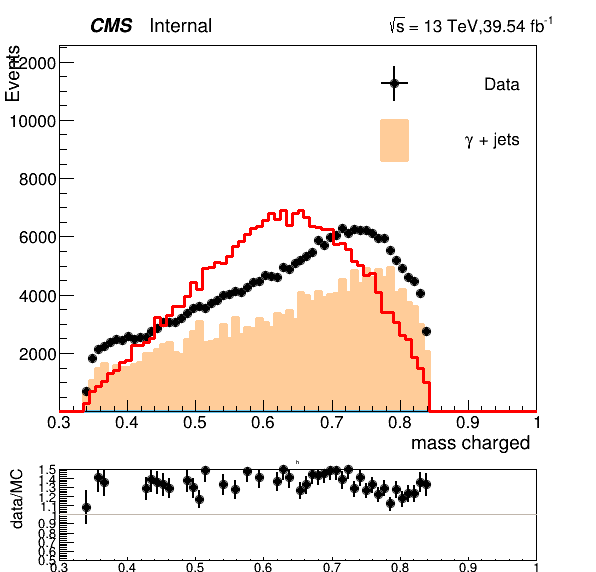
\includegraphics[width=0.45\mylength]{resources/plots/Phi3_dtrk_mass.png}
        \caption{\footnotesize (a)}
    \end{subfigure}%
    \begin{subfigure}[t]{0.50\mylength}
        \centering
        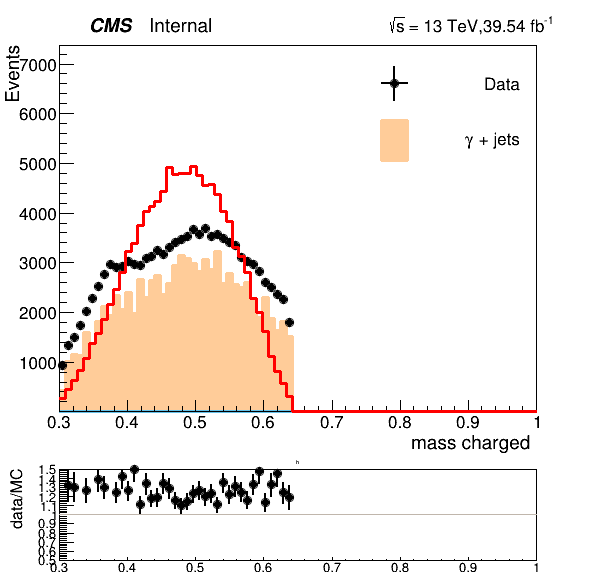
\includegraphics[width=0.45\mylength]{resources/plots/Omega_dtrk_mass.png}
        \caption{\footnotesize (b)}
    \end{subfigure}%\begin{subfigure}[t]{0.50\mylength}\baselineskip
    \vskip\baselineskip
    \vspace*{-0.1cm}
    \begin{subfigure}[t]{0.50\mylength}
        \centering
        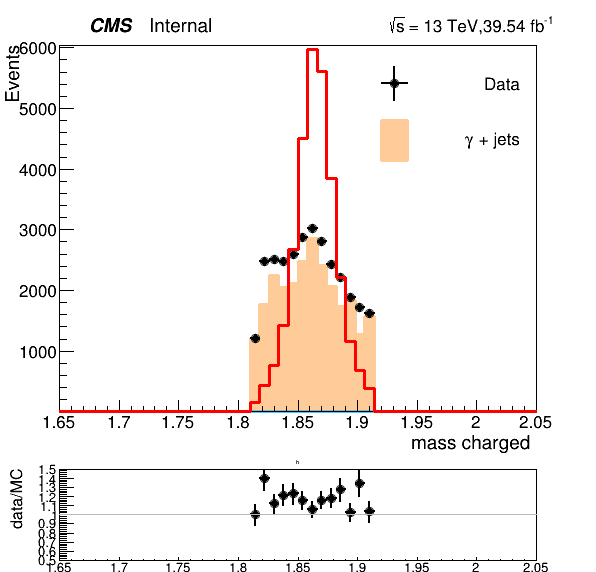
\includegraphics[width=0.45\mylength]{resources/plots/D0Star_2body_dtrk_mass.png}
        \caption{\footnotesize (c)}
    \end{subfigure}%
    \begin{subfigure}[t]{0.50\mylength}
        \centering
        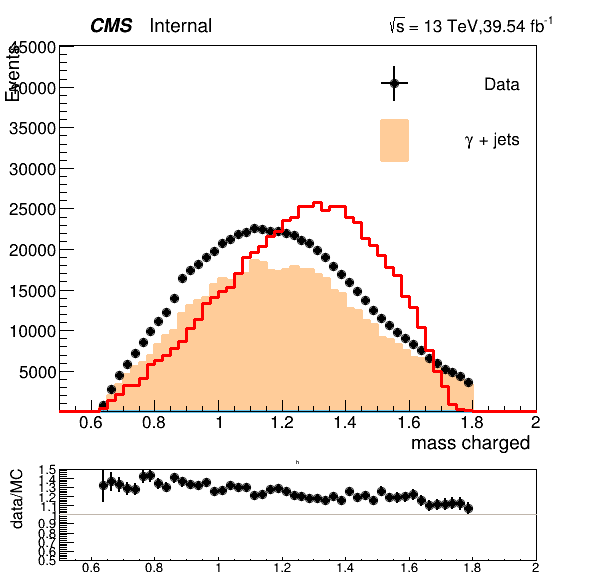
\includegraphics[width=0.45\mylength]{resources/plots/D0Star_3body_dtrk_mass.png}
        \caption{\footnotesize (d)}
    \end{subfigure}%\begin{subfigure}[t]{0.50\mylength}\baselineskip
\caption{Ditrack mass of the different studied decay modes. (a) $\phi$ channel, (b) $\omega$ channel, (c) $D^{*0}$ 2-body channel, and (d) $D^{*0}$ 3-body channel. The MC background is shown in orange, scatter points represent real data, and the signal, in red, is normalized to the data for better visualization.}
\label{fig:ditrack_mass_data}
    \vspace*{-0.0cm}
\end{figure}

Figure \ref{fig:ditrack_mass_data} displays the invariant mass of the ditrack system. In all decay channels (and in subsequent figures showing other kinematic variables), the MC background underestimates the data as it only considers the dominant contribution at LO. The data is a factor of around 20\% larger, but the estimated limits are ultimately calculated using the data for the background fit. The MC background serves the purpose of helping us comprehend the behavior of the involved processes.

In Figure \ref{fig:ditrack_mass_data} (c), a sharper resonance is observed because, as mentioned earlier, the ditrack system is a real $D^{0}$ meson. In contrast, for the other cases (where the ditrack is not a real particle), the invariant ditrack mass is considerably wider. Across all decay modes, the MC background is consistent with the data.

\begin{figure}[!ht]
    \captionsetup[subfigure]{labelformat=empty}
    \vspace*{-0.2cm}
    \centering
    \setlength{\mylength}{\textwidth}
    \begin{subfigure}[t]{0.50\mylength}
        \centering
        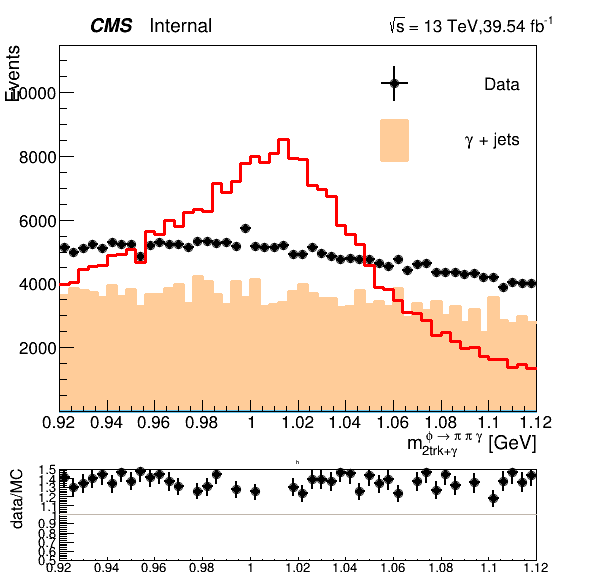
\includegraphics[width=0.45\mylength]{resources/plots/Phi3_mass.png}
        \caption{\footnotesize (a)}
    \end{subfigure}%
    \begin{subfigure}[t]{0.50\mylength}
        \centering
        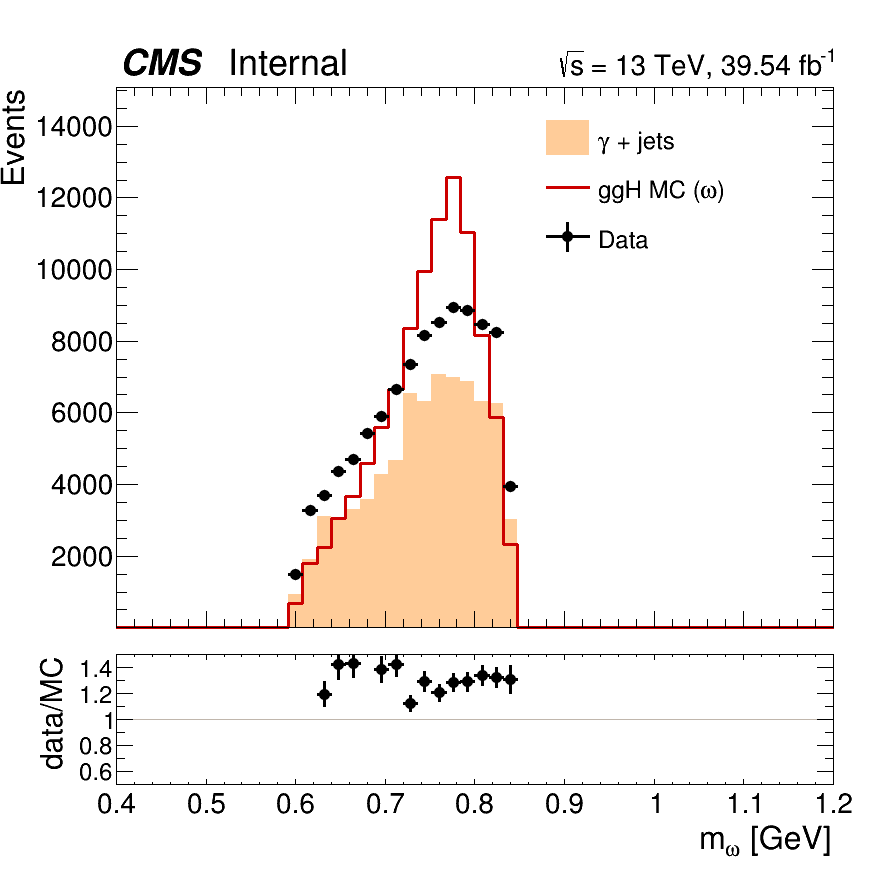
\includegraphics[width=0.45\mylength]{resources/plots/Omega_mass.png}
        \caption{\footnotesize (b)}
    \end{subfigure}%\begin{subfigure}[t]{0.50\mylength}\baselineskip
    \vskip\baselineskip
    \vspace*{-0.1cm}
    \begin{subfigure}[t]{0.50\mylength}
        \centering
        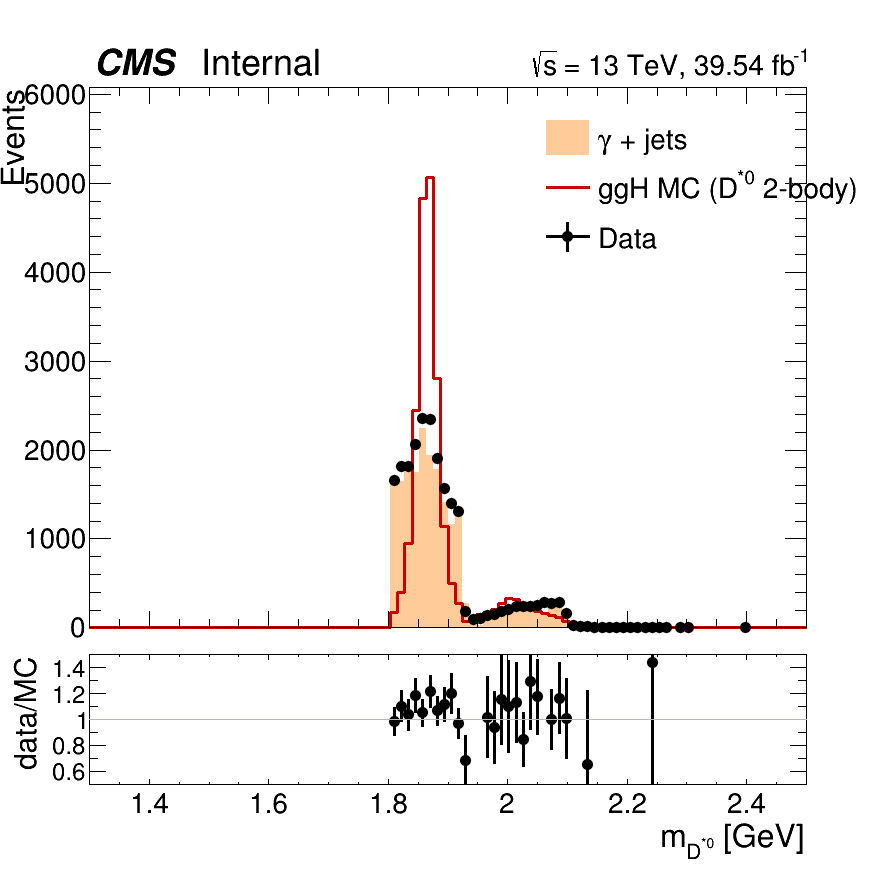
\includegraphics[width=0.45\mylength]{resources/plots/D0Star_2body_mass.png}
        \caption{\footnotesize (c)}
    \end{subfigure}%
    \begin{subfigure}[t]{0.50\mylength}
        \centering
        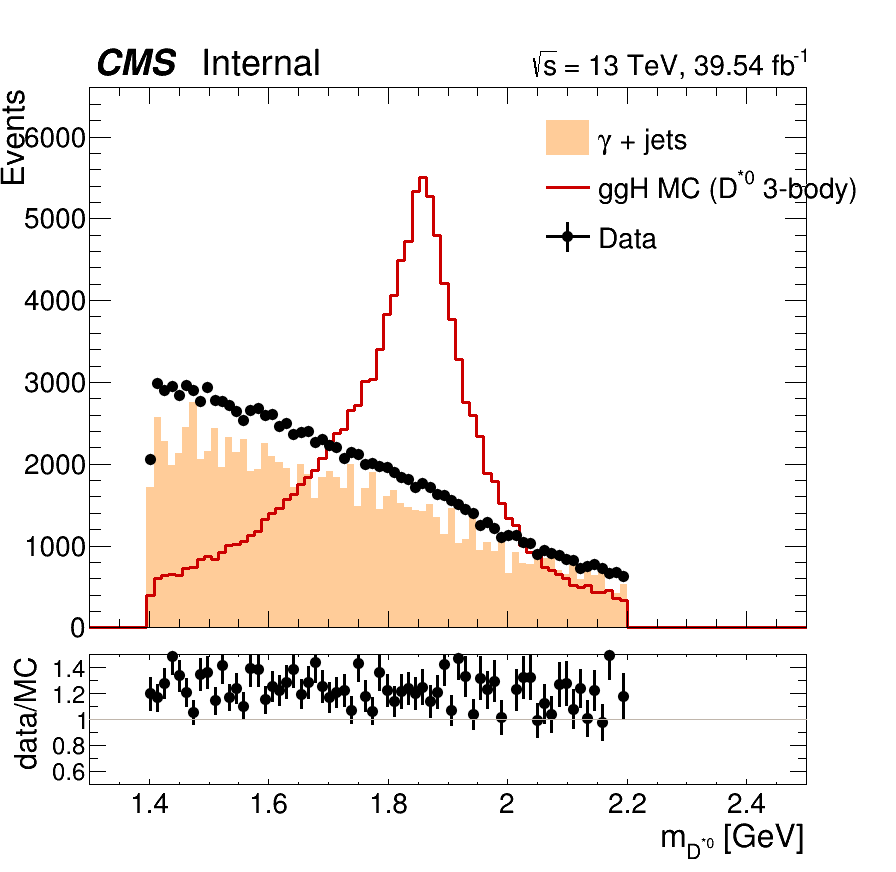
\includegraphics[width=0.45\mylength]{resources/plots/D0Star_3body_mass.png}
        \caption{\footnotesize (d)}
    \end{subfigure}%\begin{subfigure}[t]{0.50\mylength}\baselineskip
\caption{Full meson's mass of the different studied decay modes. (a) $\phi$ channel, (b) $\omega$ channel, (c) $D^{*0}$ 2-body channel, and (d) $D^{*0}$ 3-body channel. The MC background is shown in orange, scatter points represent real data, and the signal, in red, is normalized to the data for better visualization.}
\label{fig:full_mass_data}
    \vspace*{-0.0cm}
\end{figure}

Figure \ref{fig:full_mass_data} displays the mass of the full meson. This variable is sharper than the ditrack system's mass in all channels because it consists of a real meson. However, for the $D^{*0}$ 2-body decay mode, it is not well reconstructed. In approximately $\sim 87\%$ of events, no photon compatible with the decay of a neutral particle is recovered, and therefore the computed full mass is the same as the ditrack system's mass. This is why this variable is not used in the BDT for regressing the transverse momentum (see Section \ref{sec:meson_reconstruction}). All decay modes exhibit missing energy, as all channels have an asymmetric left shoulder.

\begin{figure}[!ht]
    \captionsetup[subfigure]{labelformat=empty}
    \vspace*{-0.2cm}
    \centering
    \setlength{\mylength}{\textwidth}
    \begin{subfigure}[t]{0.50\mylength}
        \centering
        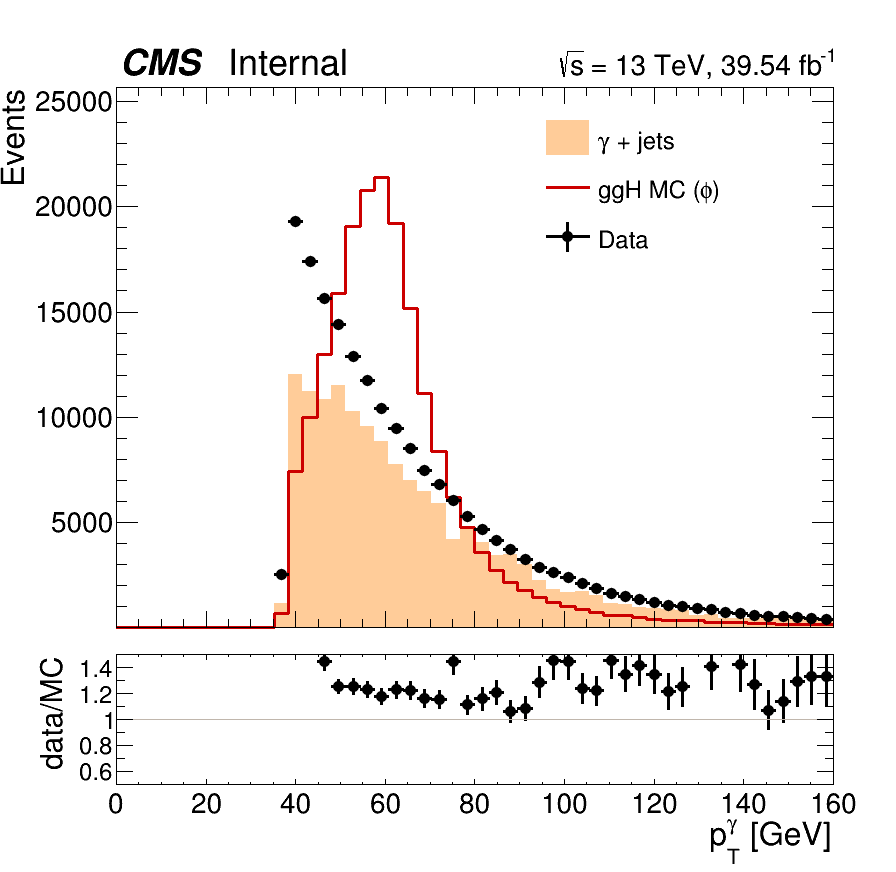
\includegraphics[width=0.45\mylength]{resources/plots/Phi3_photon_pt.png}
        \caption{\footnotesize (a)}
    \end{subfigure}%
    \begin{subfigure}[t]{0.50\mylength}
        \centering
        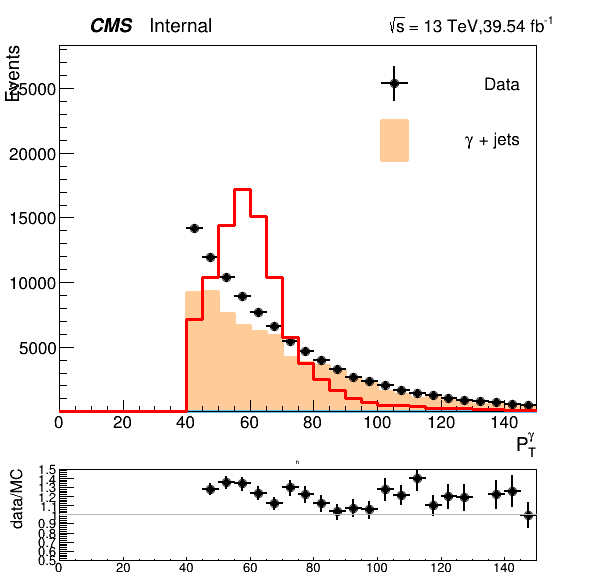
\includegraphics[width=0.45\mylength]{resources/plots/Omega_photon_pt.png}
        \caption{\footnotesize (b)}
    \end{subfigure}%\begin{subfigure}[t]{0.50\mylength}\baselineskip
    \vskip\baselineskip
    \vspace*{-0.1cm}
    \begin{subfigure}[t]{0.50\mylength}
        \centering
        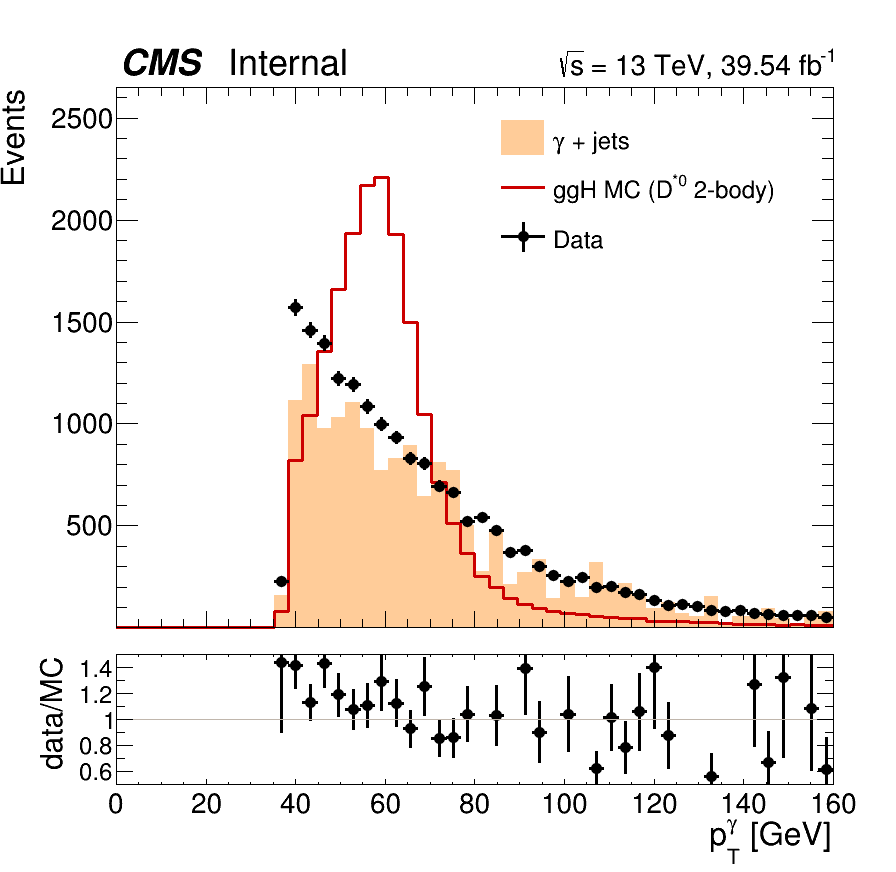
\includegraphics[width=0.45\mylength]{resources/plots/D0Star_2body_photon_pt.png}
        \caption{\footnotesize (c)}
    \end{subfigure}%
    \begin{subfigure}[t]{0.50\mylength}
        \centering
        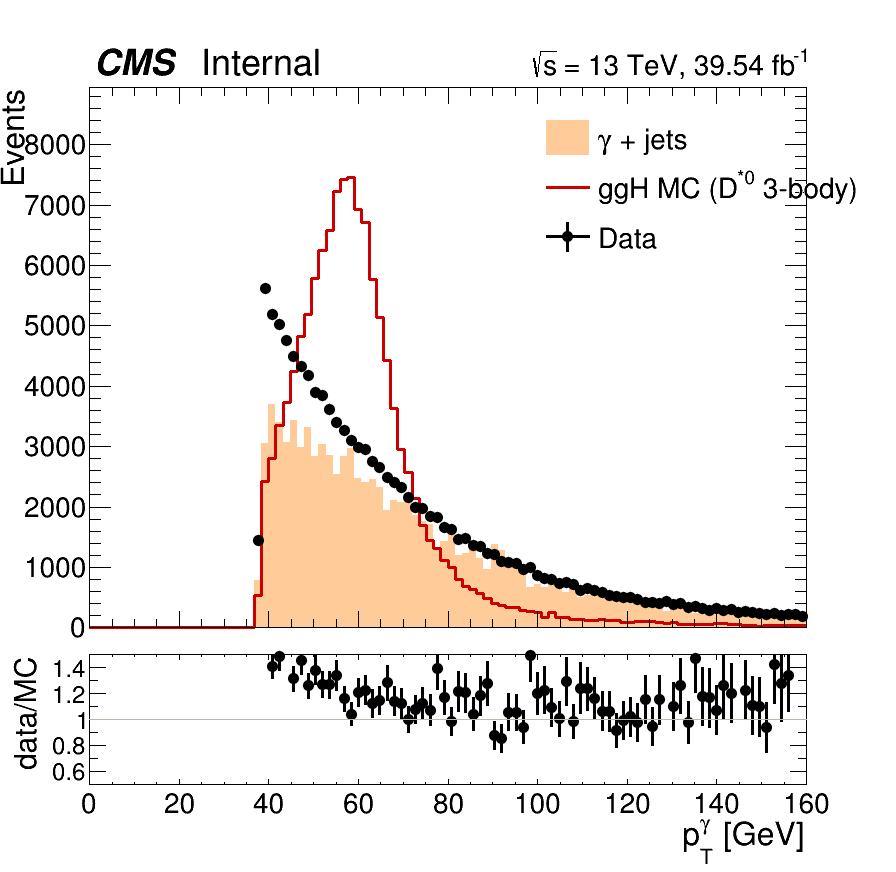
\includegraphics[width=0.45\mylength]{resources/plots/D0Star_3body_photon_pt.png}
        \caption{\footnotesize (d)}
    \end{subfigure}%\begin{subfigure}[t]{0.50\mylength}\baselineskip
\caption{Transverse momentum $\pT$ of the primary photon from the Higgs boson decay, for the different studied decay modes. (a) $\phi$ channel, (b) $\omega$ channel, (c) $D^{*0}$ 2-body channel, and (d) $D^{*0}$ 3-body channel. The MC background is shown in orange, scatter points represent real data, and the signal, in red, is normalized to the data for better visualization.}
\label{fig:photon_pt_data}
    \vspace*{-0.0cm}
\end{figure}

Figure \ref{fig:photon_pt_data} presents the transverse momentum of the primary photon originating directly from the Higgs boson decay. The signal peaks at around 60 GeV for all channels, which is roughly half of the Higgs boson's mass. This is consistent with Figure \ref{fig:full_pt_data}, which shows the transverse momentum of each meson. In every channel, the signal also peaks around 60 GeV, which with the transverse momentum of the photon adds up to the 125 GeV of the Higgs boson's mass.

\begin{figure}[!ht]
    \captionsetup[subfigure]{labelformat=empty}
    \vspace*{-0.2cm}
    \centering
    \setlength{\mylength}{\textwidth}
    \begin{subfigure}[t]{0.50\mylength}
        \centering
        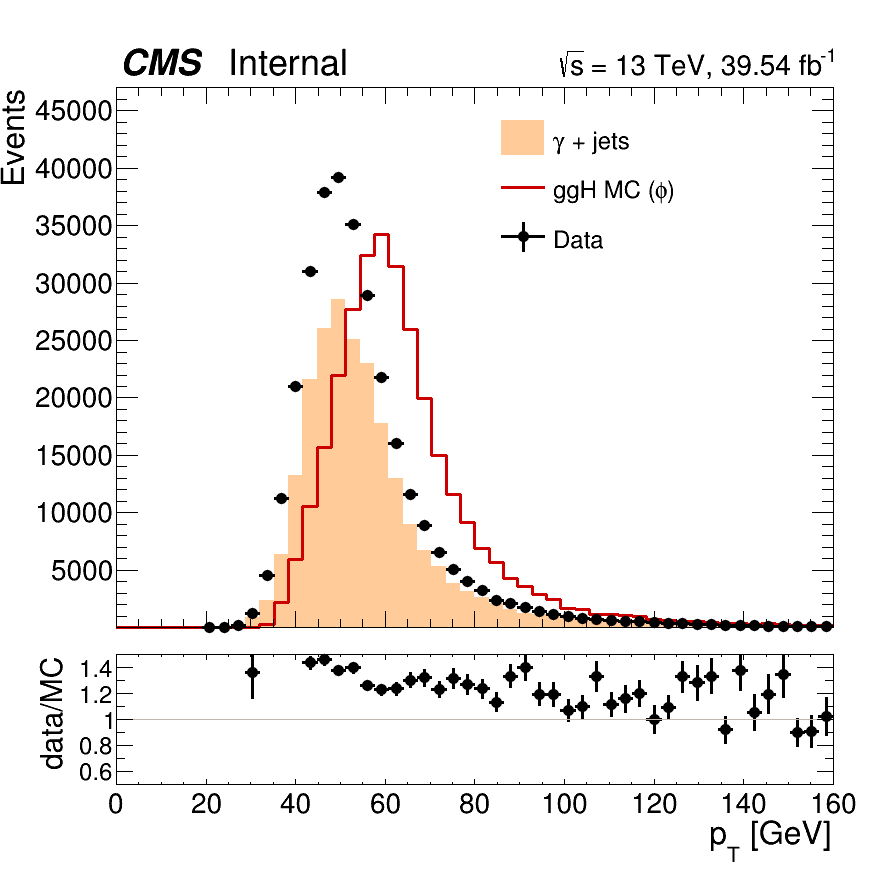
\includegraphics[width=0.45\mylength]{resources/plots/Phi3_pt.png}
        \caption{\footnotesize (a)}
    \end{subfigure}%
    \begin{subfigure}[t]{0.50\mylength}
        \centering
        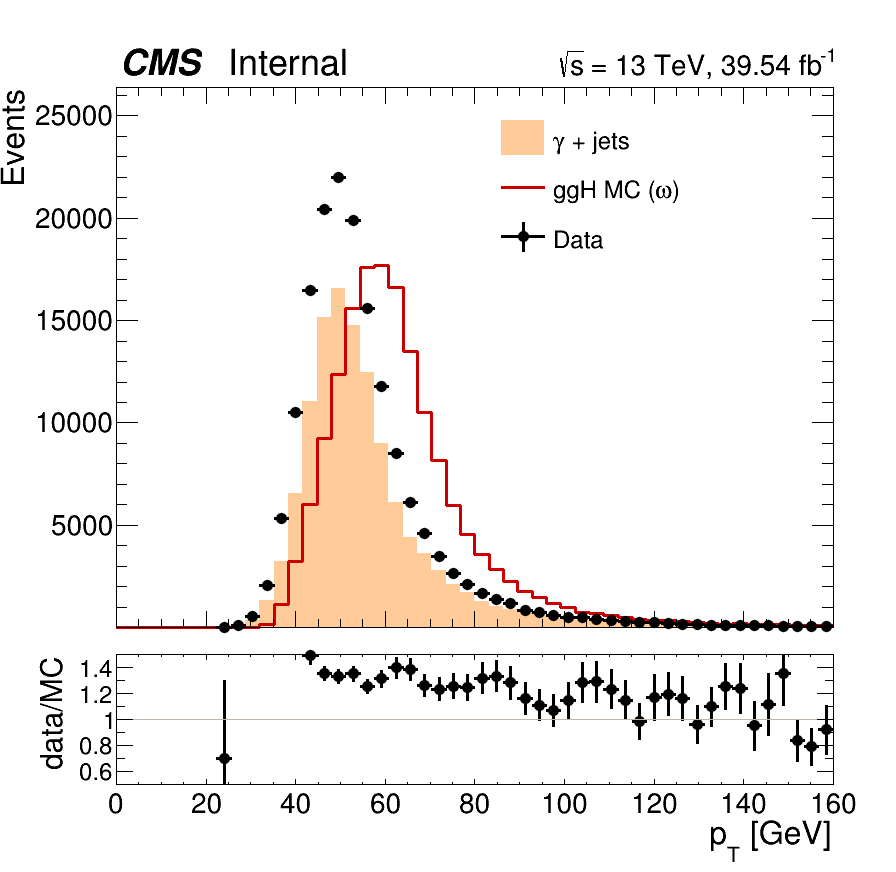
\includegraphics[width=0.45\mylength]{resources/plots/Omega_pt.png}
        \caption{\footnotesize (b)}
    \end{subfigure}%\begin{subfigure}[t]{0.50\mylength}\baselineskip
    \vskip\baselineskip
    \vspace*{-0.1cm}
    \begin{subfigure}[t]{0.50\mylength}
        \centering
        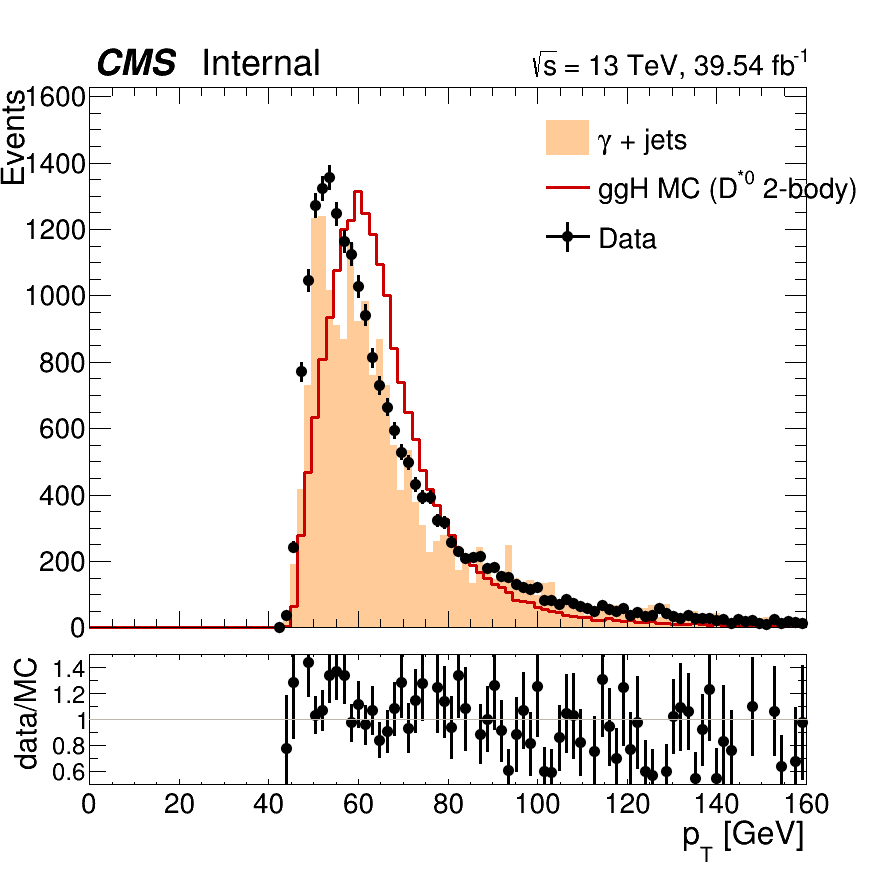
\includegraphics[width=0.45\mylength]{resources/plots/D0Star_2body_pt.png}
        \caption{\footnotesize (c)}
    \end{subfigure}%
    \begin{subfigure}[t]{0.50\mylength}
        \centering
        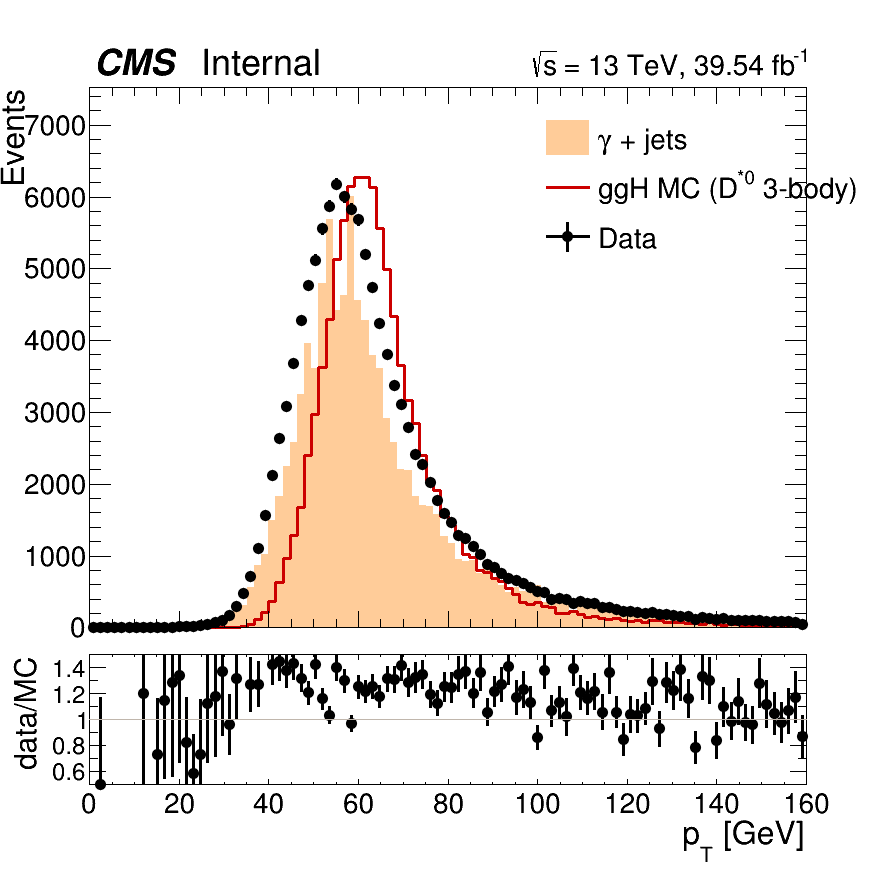
\includegraphics[width=0.45\mylength]{resources/plots/D0Star_3body_pt.png}
        \caption{\footnotesize (d)}
    \end{subfigure}%\begin{subfigure}[t]{0.50\mylength}\baselineskip
\caption{Transverse momentum $\pT$ of the full meson for the different studied decay modes. (a) $\phi$ channel, (b) $\omega$ channel, (c) $D^{*0}$ 2-body channel, and (d) $D^{*0}$ 3-body channel. The MC background is shown in orange, scatter points represent real data, and the signal, in red, is normalized to the data for better visualization.}
\label{fig:full_pt_data}
    \vspace*{-0.0cm}
\end{figure}

\begin{figure}[!ht]
    \captionsetup[subfigure]{labelformat=empty}
    \vspace*{-0.2cm}
    \centering
    \setlength{\mylength}{\textwidth}
    \begin{subfigure}[t]{0.50\mylength}
        \centering
        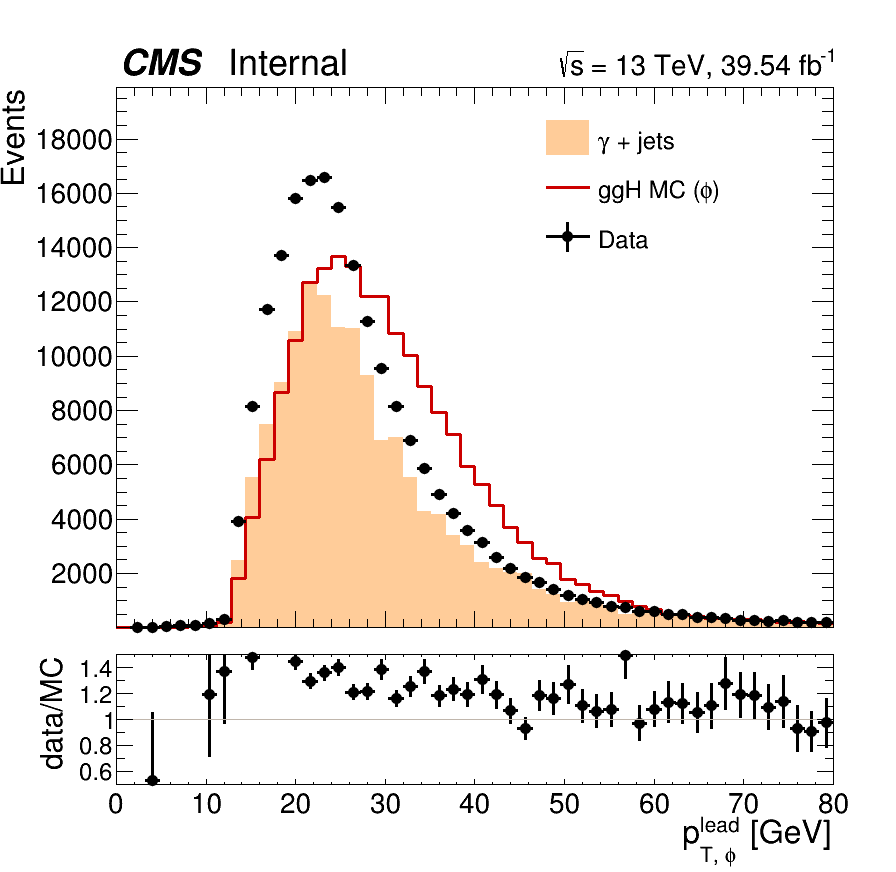
\includegraphics[width=0.45\mylength]{resources/plots/Phi3_lead_pt.png}
        \caption{\footnotesize (a)}
    \end{subfigure}%
    \begin{subfigure}[t]{0.50\mylength}
        \centering
        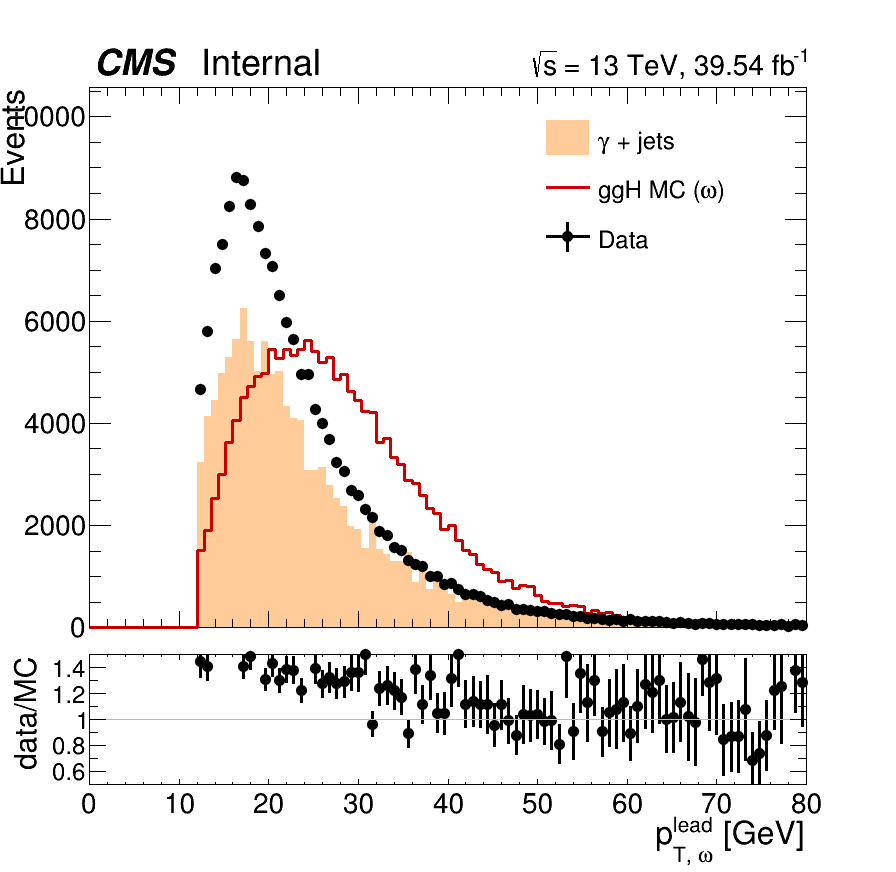
\includegraphics[width=0.45\mylength]{resources/plots/Omega_lead_pt.png}
        \caption{\footnotesize (b)}
    \end{subfigure}%\begin{subfigure}[t]{0.50\mylength}\baselineskip
    \vskip\baselineskip
    \vspace*{-0.1cm}
    \begin{subfigure}[t]{0.50\mylength}
        \centering
        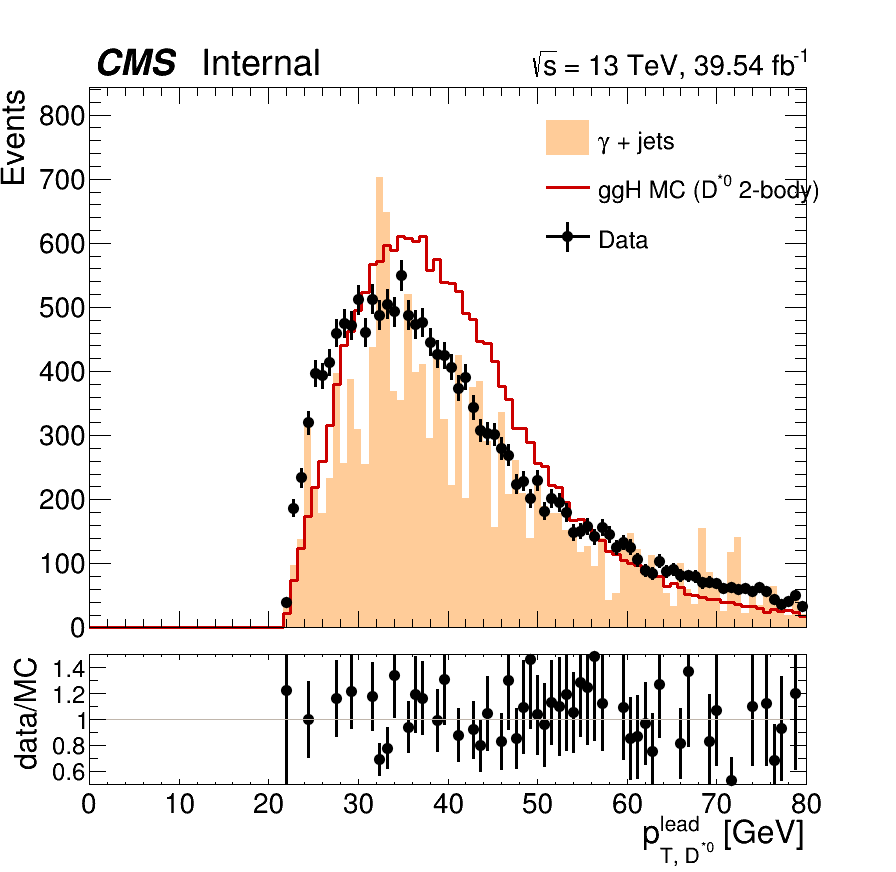
\includegraphics[width=0.45\mylength]{resources/plots/D0Star_2body_lead_pt.png}
        \caption{\footnotesize (c)}
    \end{subfigure}%
    \begin{subfigure}[t]{0.50\mylength}
        \centering
        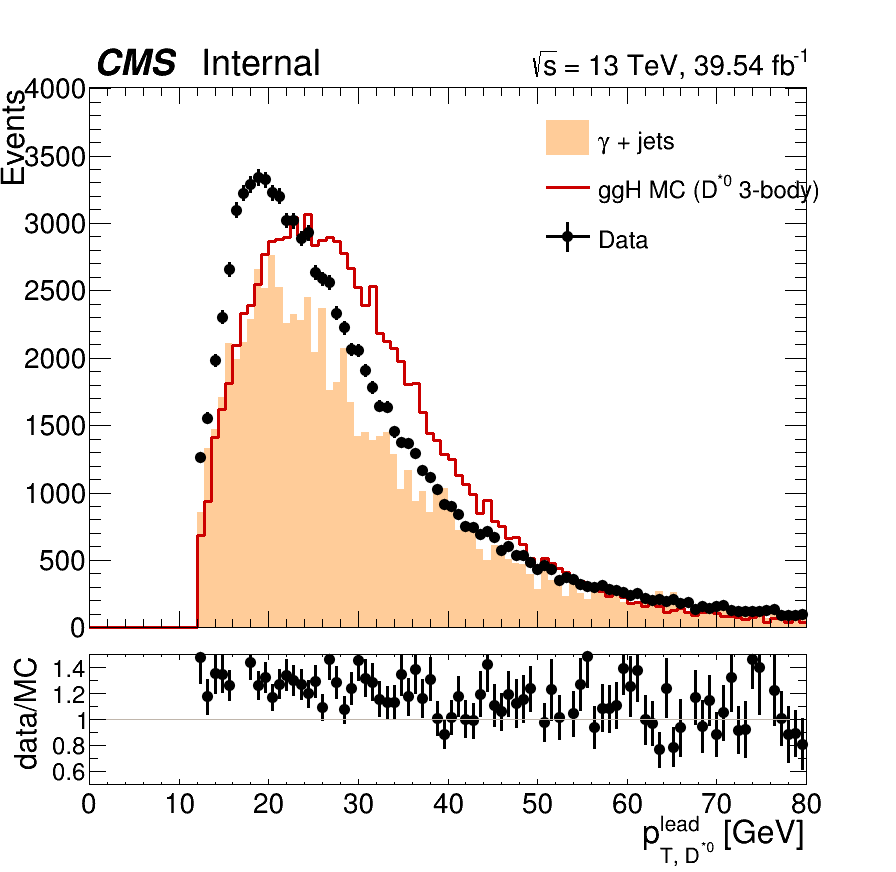
\includegraphics[width=0.45\mylength]{resources/plots/D0Star_3body_lead_pt.png}
        \caption{\footnotesize (d)}
    \end{subfigure}%\begin{subfigure}[t]{0.50\mylength}\baselineskip
\caption{Transverse momentum $\pT$ of the leading charged track for the different studied decay modes. (a) $\phi$ channel, (b) $\omega$ channel, (c) $D^{*0}$ 2-body channel, and (d) $D^{*0}$ 3-body channel. The MC background is shown in orange, scatter points represent real data, and the signal, in red, is normalized to the data for better visualization.}
\label{fig:lead_pt_data}
    \vspace*{-0.0cm}
\end{figure}

\newpage

Figures \ref{fig:lead_pt_data} and \ref{fig:sublead_pt_data} illustrate the transverse momentum of the charged leading and subleading tracks for each decay mode. All channels show a similar shape for the signal. However, it is worth noting that in the $D^{*0}$ 2-body decay, both the leading and subleading tracks are more energetic, as this is the only scenario where $D^{0}$ decays into only two charged tracks (the neutral particle from $D^{*0}\decaysto D^{0}\pi^{0}/\gamma$ typically carries around $\sim5$ GeV in energy).

\begin{figure}[!ht]
    \captionsetup[subfigure]{labelformat=empty}
    \vspace*{-0.2cm}
    \centering
    \setlength{\mylength}{\textwidth}
    \begin{subfigure}[t]{0.50\mylength}
        \centering
        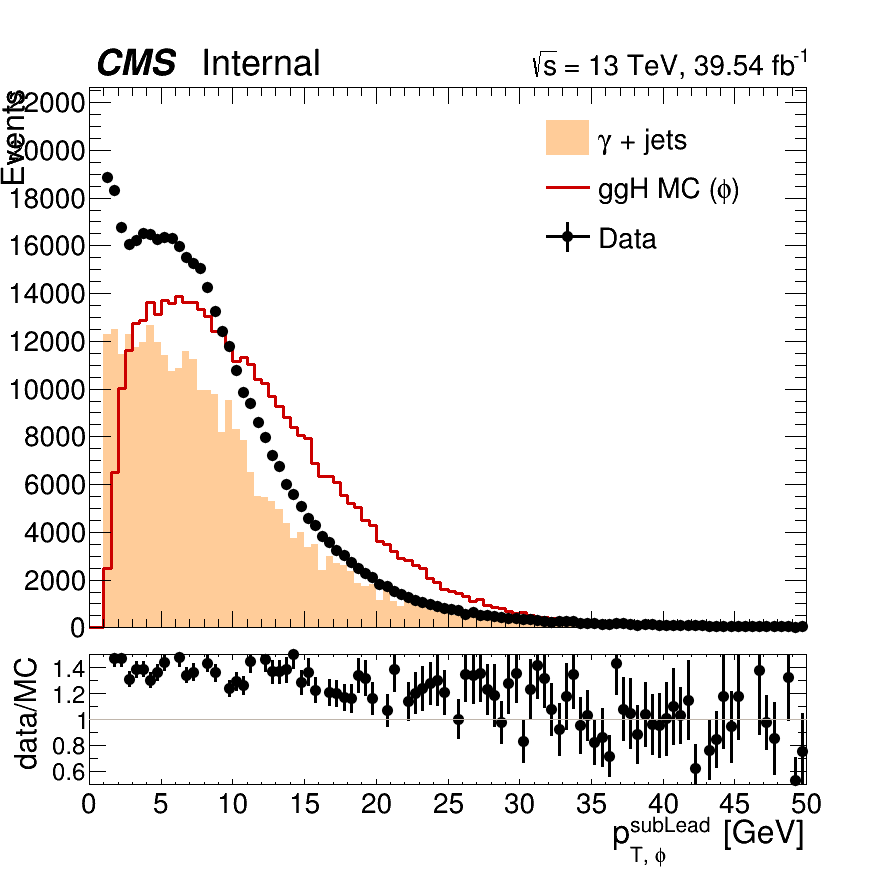
\includegraphics[width=0.45\mylength]{resources/plots/Phi3_sublead_pt.png}
        \caption{\footnotesize (a)}
    \end{subfigure}%
    \begin{subfigure}[t]{0.50\mylength}
        \centering
        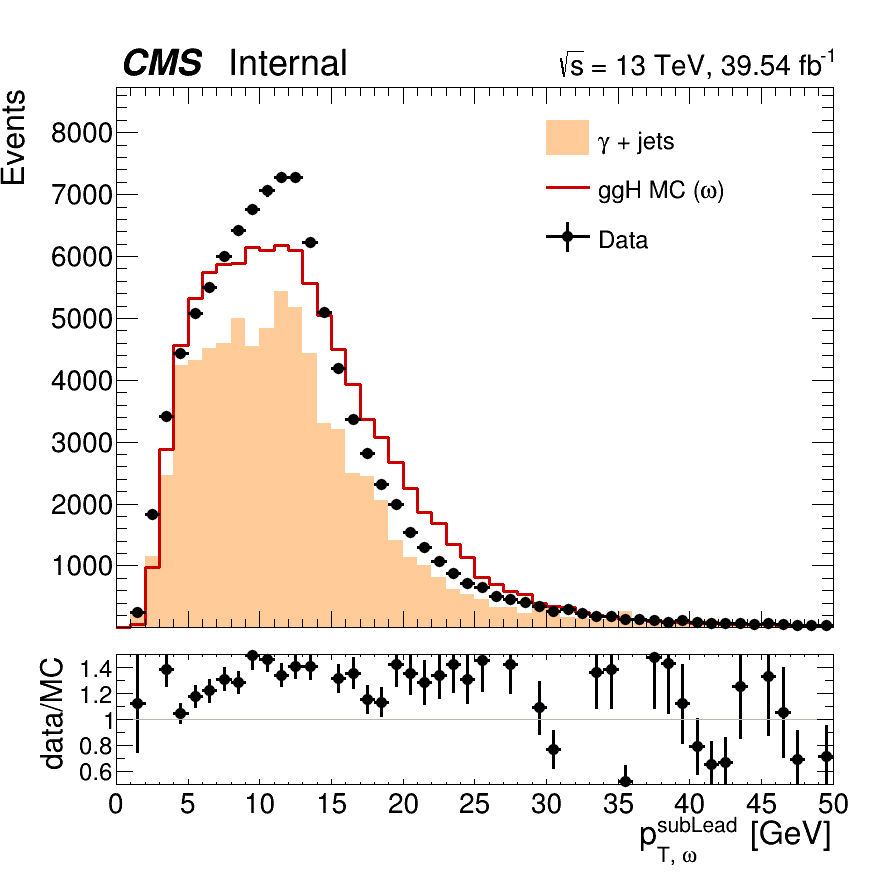
\includegraphics[width=0.45\mylength]{resources/plots/Omega_sublead_pt.png}
        \caption{\footnotesize (b)}
    \end{subfigure}%\begin{subfigure}[t]{0.50\mylength}\baselineskip
    \vskip\baselineskip
    \vspace*{-0.1cm}
    \begin{subfigure}[t]{0.50\mylength}
        \centering
        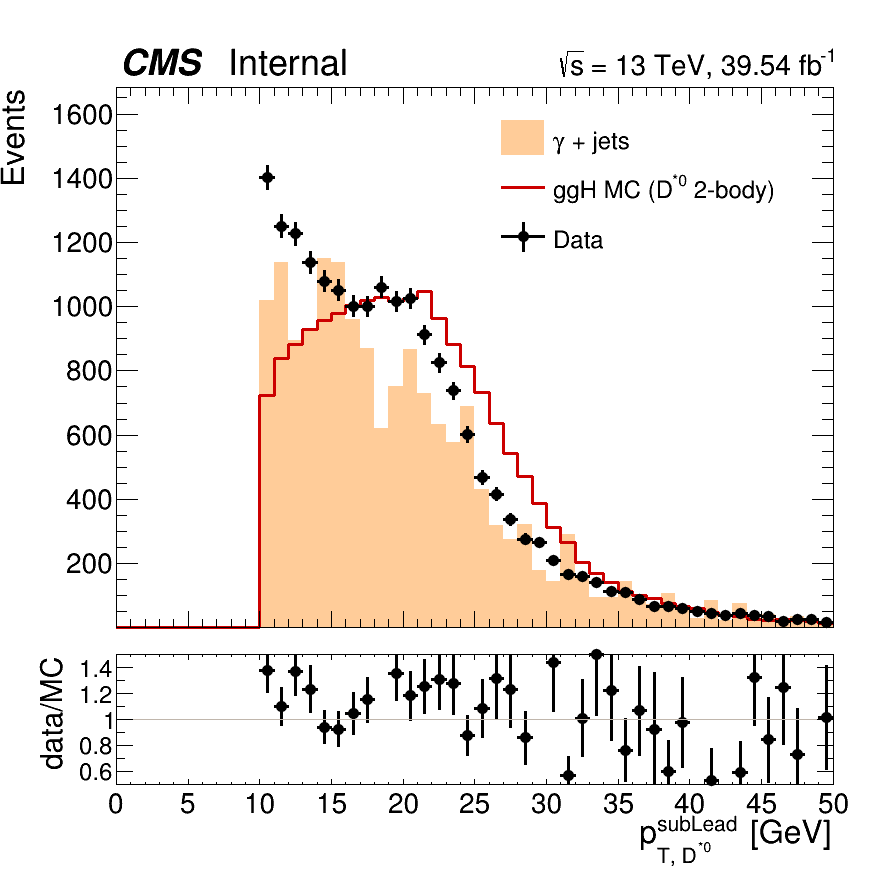
\includegraphics[width=0.45\mylength]{resources/plots/D0Star_2body_sublead_pt.png}
        \caption{\footnotesize (c)}
    \end{subfigure}%
    \begin{subfigure}[t]{0.50\mylength}
        \centering
        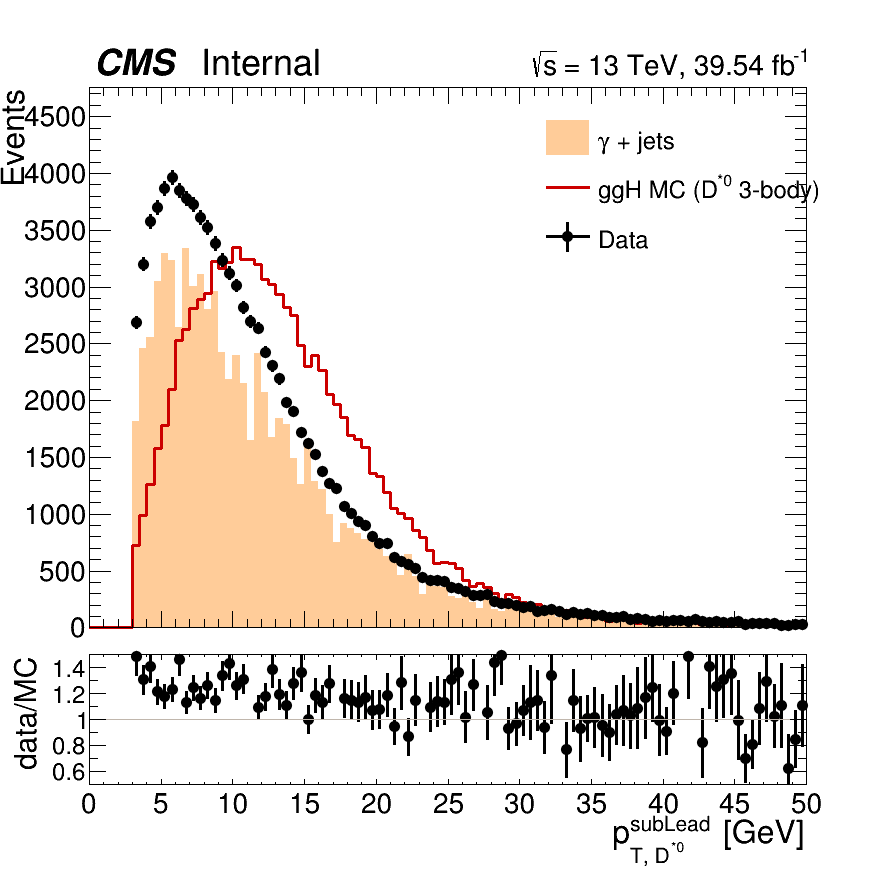
\includegraphics[width=0.45\mylength]{resources/plots/D0Star_3body_sublead_pt.png}
        \caption{\footnotesize (d)}
    \end{subfigure}%\begin{subfigure}[t]{0.50\mylength}\baselineskip
\caption{Transverse momentum $\pT$ of the subleading charged track for the different studied decay modes. (a) $\phi$ channel, (b) $\omega$ channel, (c) $D^{*0}$ 2-body channel, and (d) $D^{*0}$ 3-body channel. The MC background is shown in orange, scatter points represent real data, and the signal, in red, is normalized to the data for better visualization.}
\label{fig:sublead_pt_data}
    \vspace*{-0.0cm}
\end{figure}

\section{Signal and background modelling \todo{ADD 2D FIT}}\label{sec:modelling}

The potential Higgs boson signal is obtained by fitting the invariant mass distribution $M_{\gamma, M}$ for each decay mode separately, since the signal is expected to show a peak over a monotonous background. Both the signal and background are directly estimated from MC (signal) or data (background) by fitting the photon-meson mass spectrum with analytical functions. The RooFit framework \cite{CERN:root_roofit}, a toolkit provided within the ROOT module for modeling the expected event distribution, is used for this purpose, and a binned maximum likelihood fit is conducted.
\begin{figure}[!ht]
    \captionsetup[subfigure]{labelformat=empty}
    \vspace*{-0.2cm}
    \centering
    \setlength{\mylength}{\textwidth}
    \begin{subfigure}[t]{0.50\mylength}
        \centering
        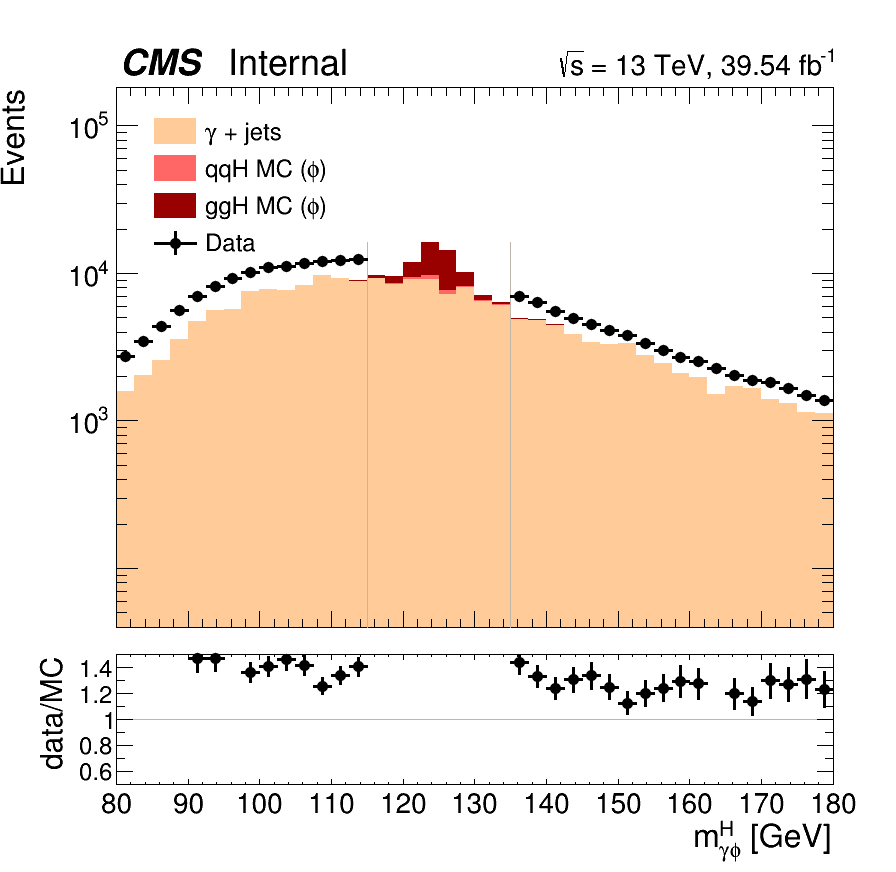
\includegraphics[width=0.45\mylength]{resources/plots/Phi3_HiggsMass.png}
        \caption{\footnotesize (a)}
    \end{subfigure}%
    \begin{subfigure}[t]{0.50\mylength}
        \centering
        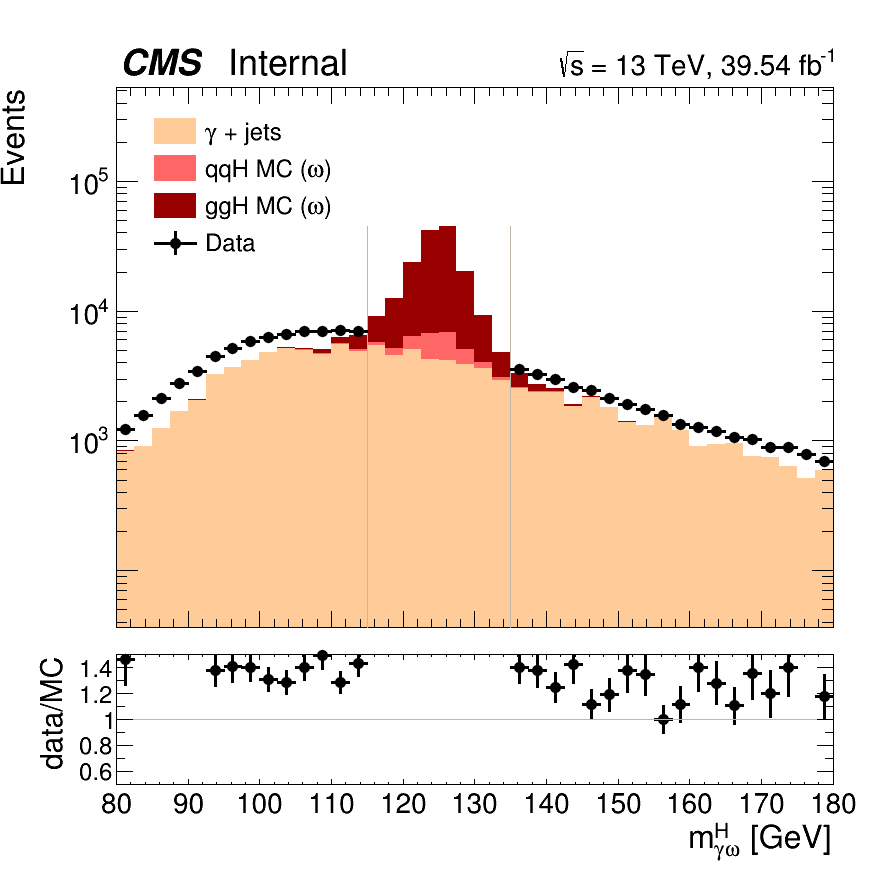
\includegraphics[width=0.45\mylength]{resources/plots/Omega_HiggsMass.png}
        \caption{\footnotesize (b)}
    \end{subfigure}%\begin{subfigure}[t]{0.50\mylength}\baselineski
    \vskip\baselineskip
    \vspace*{-0.1cm}
    \begin{subfigure}[t]{0.50\mylength}
        \centering
        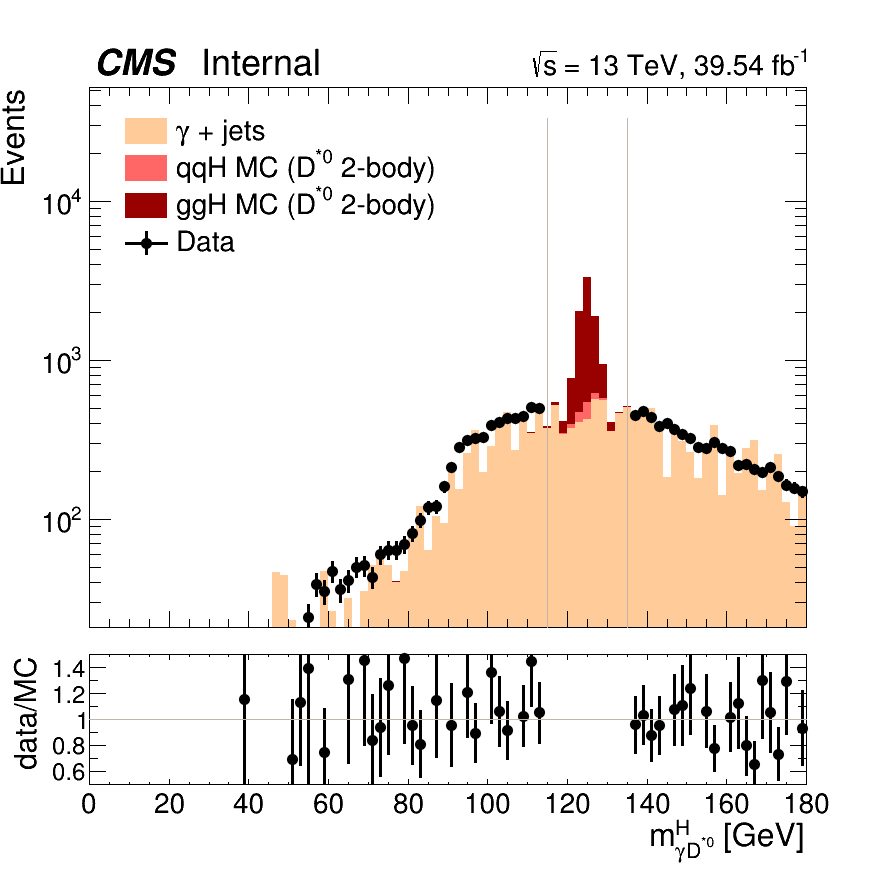
\includegraphics[width=0.45\mylength]{resources/plots/D0Star_2body_HiggsMass.png}
        \caption{\footnotesize (c)}
    \end{subfigure}%
    \begin{subfigure}[t]{0.50\mylength}
        \centering
        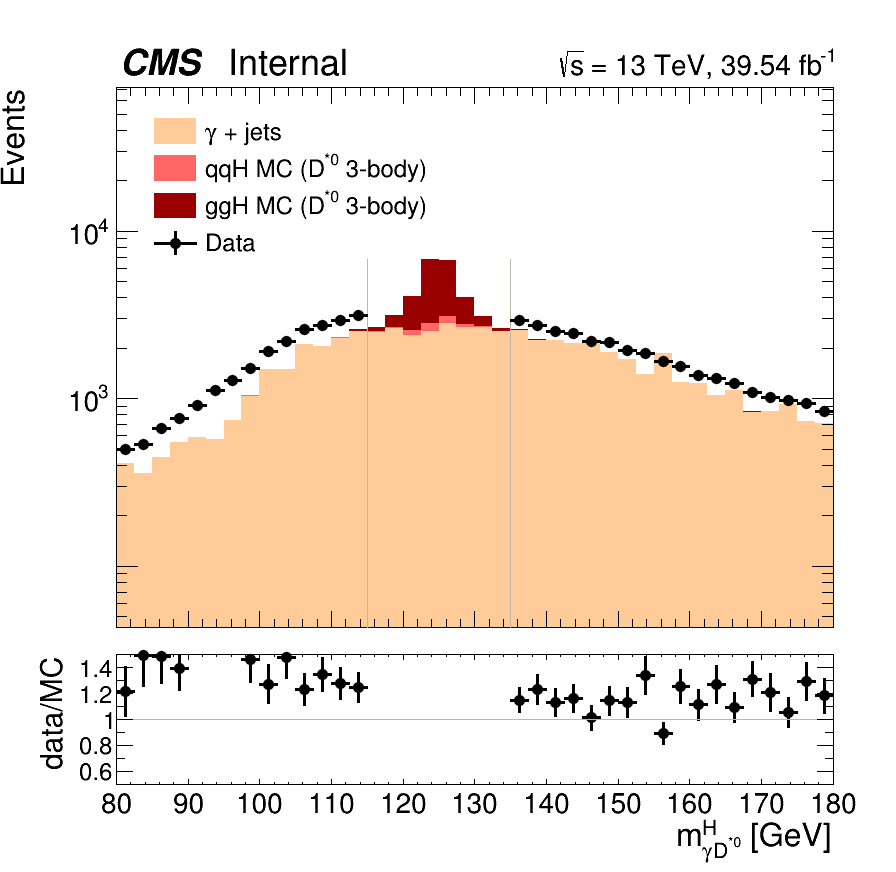
\includegraphics[width=0.45\mylength]{resources/plots/D0Star_3body_HiggsMass.png}
        \caption{\footnotesize (d)}
    \end{subfigure}%\begin{subfigure}[t]{0.50\mylength}\baselineskip
\caption{Higgs invariant mass distribution $M_{\gamma, M}$ for the different studied decay modes. (a) $\phi$ channel, (b) $\omega$ channel, (c) $D^{*0}$ 2-body channel, and (d) $D^{*0}$ 3-body channel. The MC background is shown in orange, scatter points represent real data, and the signal, in crimson, is scaled {\r to what ???} for better visualization.}
\label{fig:Higgs_mass_data}
    \vspace*{-0.0cm}
\end{figure}
Figure \ref{fig:Higgs_mass_data} displays the photon-meson invariant mass distribution for each channel. The data in the region of interest is not shown, it is still \textit{blinded}. Only after completing the full analysis and ensuring the consistency of the techniques used can the data be unblinded to enable actual measurements. This approach is commonly employed in high-energy physics to maintain an unbiased study.

Based on the earlier discussed selection criteria, the shape of this background exhibits a turn-on structure in $M_{\gamma, M}$. This turn-on varies for each decay mode due to the kinematic constraints of the events and the imposed selection cuts.

\subsection*{Signal modelling}

Although previously discussed, it is worth emphasizing that analysis sensitivity relies on the resolution of the photon-meson mass $M_{\gamma, M}$, which strongly depends on the kinematics, especially the transverse momentum of the photon/meson.

The expected photon-meson mass candidate distribution in signal events, for each decay mode, is modeled using a double-sided Crystal Ball. This function, named after the Crystal Ball Collaboration \cite{A2:CB}, is a probability density function (PDF) commonly employed in high-energy physics (HEP). It consists of a Gaussian center and two asymmetric tails modeled by power-law functions, and it is $\mathcal{C}^{1}$, i.e., continuous with a continuous derivative. This functional form simultaneously offers a robust description of the Higgs boson mass spectrum and a straightforward way to incorporate shape uncertainties, as it has only one parameter associated with the peak and two with the width of the lineshape. The tails are necessary to account for the non-Gaussian response of the photons and meson. Further information about this PDF and its implementation in ROOT is available in Ref. \cite{CERN:root_CB}.

\subsection*{Background modelling}

The monotonous $M_{\gamma, M}$ background distribution is estimated by fitting the photon-meson mass spectrum in the signal fit region ($100 < M_{\gamma, M} < 160\ \GeV$) using analytic functions. Two side bands, $100 < M_{\gamma, M} < 115\ \GeV$ and $135 < M_{\gamma, M} < 160\ \GeV$, are used to constrain the background fit. Multiple functions are used to address the incomplete model knowledge. These will be part of the final fit to take into account the uncertainty in the background model choice and to estimate the bias from selecting a specific background parameterization. The set of functions consists of Bernestein and Chebychev Polynomials.

No prior knowledge of the parameters of the fit functions (in both shape and normalization) is assumed, i.e. they are allowed to vary freely in the data fit. Table \ref{tab:bkg_polynomials} reports the degrees of freedom (dof) and $\chi^2$/dof for both polynomial classes and for each decay mode.
\begin{table}[!ht]
    \centering
    \begin{tabular}{|l|c|c|}
        \hline
        \cellcolor{lightgray}Decay channel & \cellcolor{lightgray}Bernestein & \cellcolor{lightgray}Chebychev \\ \hline
        $\phi$          &\r4-dof, $\chi^2$/dof=0.75   &\r4-dof, $\chi^2$/dof=0.75   \\
        $\omega$        &\r4-dof, $\chi^2$/dof=0.75   &\r4-dof, $\chi^2$/dof=0.75   \\
        $D^{*0}$ 2-body &\r4-dof, $\chi^2$/dof=0.75   &\r4-dof, $\chi^2$/dof=0.75   \\
        $D^{*0}$ 3-body &\r4-dof, $\chi^2$/dof=0.75   &\r4-dof, $\chi^2$/dof=0.75   \\
        \hline
        \end{tabular}
    \caption{Degrees of freedom and $\chi^2$/dof for each decay mode and polynomial type used to model the background photon-meson mass spectrum $M_{\gamma, M}$.}
    \label{tab:bkg_polynomials}
\end{table}

Figures \ref{fig:sig_bkg_modelling_phi_omega} and \ref{fig:sig_bkg_modelling_d0star} show the MC signal and data (for the background estimation) for each channel, with the fitted models. \todo{Discuss plots Figures \ref{fig:sig_bkg_modelling_phi_omega} and \ref{fig:sig_bkg_modelling_d0star} further when sidebands are in place.}

\begin{figure}[!ht]
    \captionsetup[subfigure]{labelformat=empty}
    \vspace*{-0.2cm}
    \centering
    \setlength{\mylength}{\textwidth}
    \begin{subfigure}[t]{0.50\mylength}
        \centering
        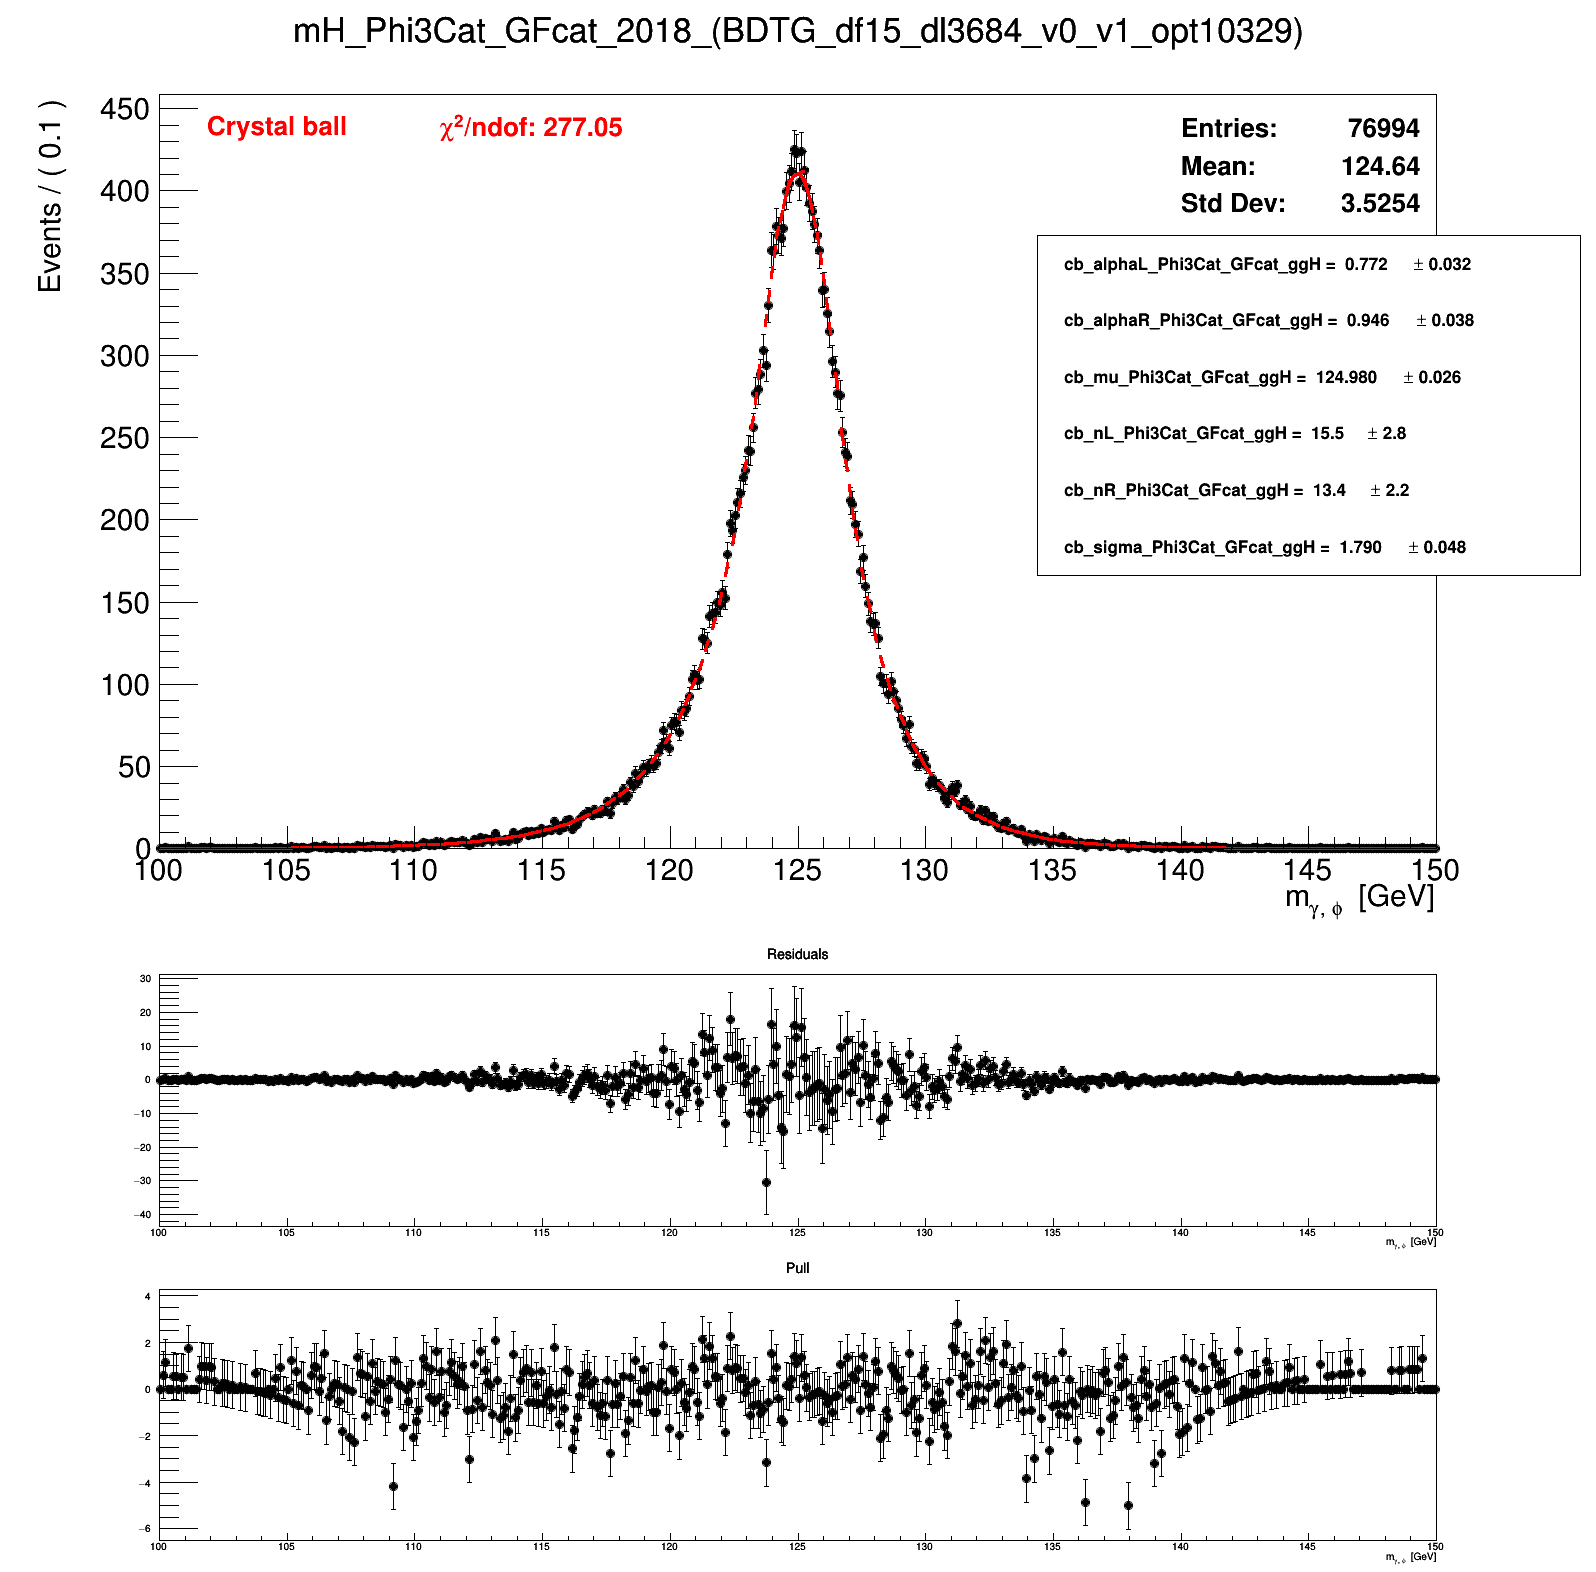
\includegraphics[width=0.45\mylength]{resources/plots/Phi3_fit_SGN.png}
        \caption{\footnotesize (a)}
    \end{subfigure}%
    \begin{subfigure}[t]{0.50\mylength}
        \centering
        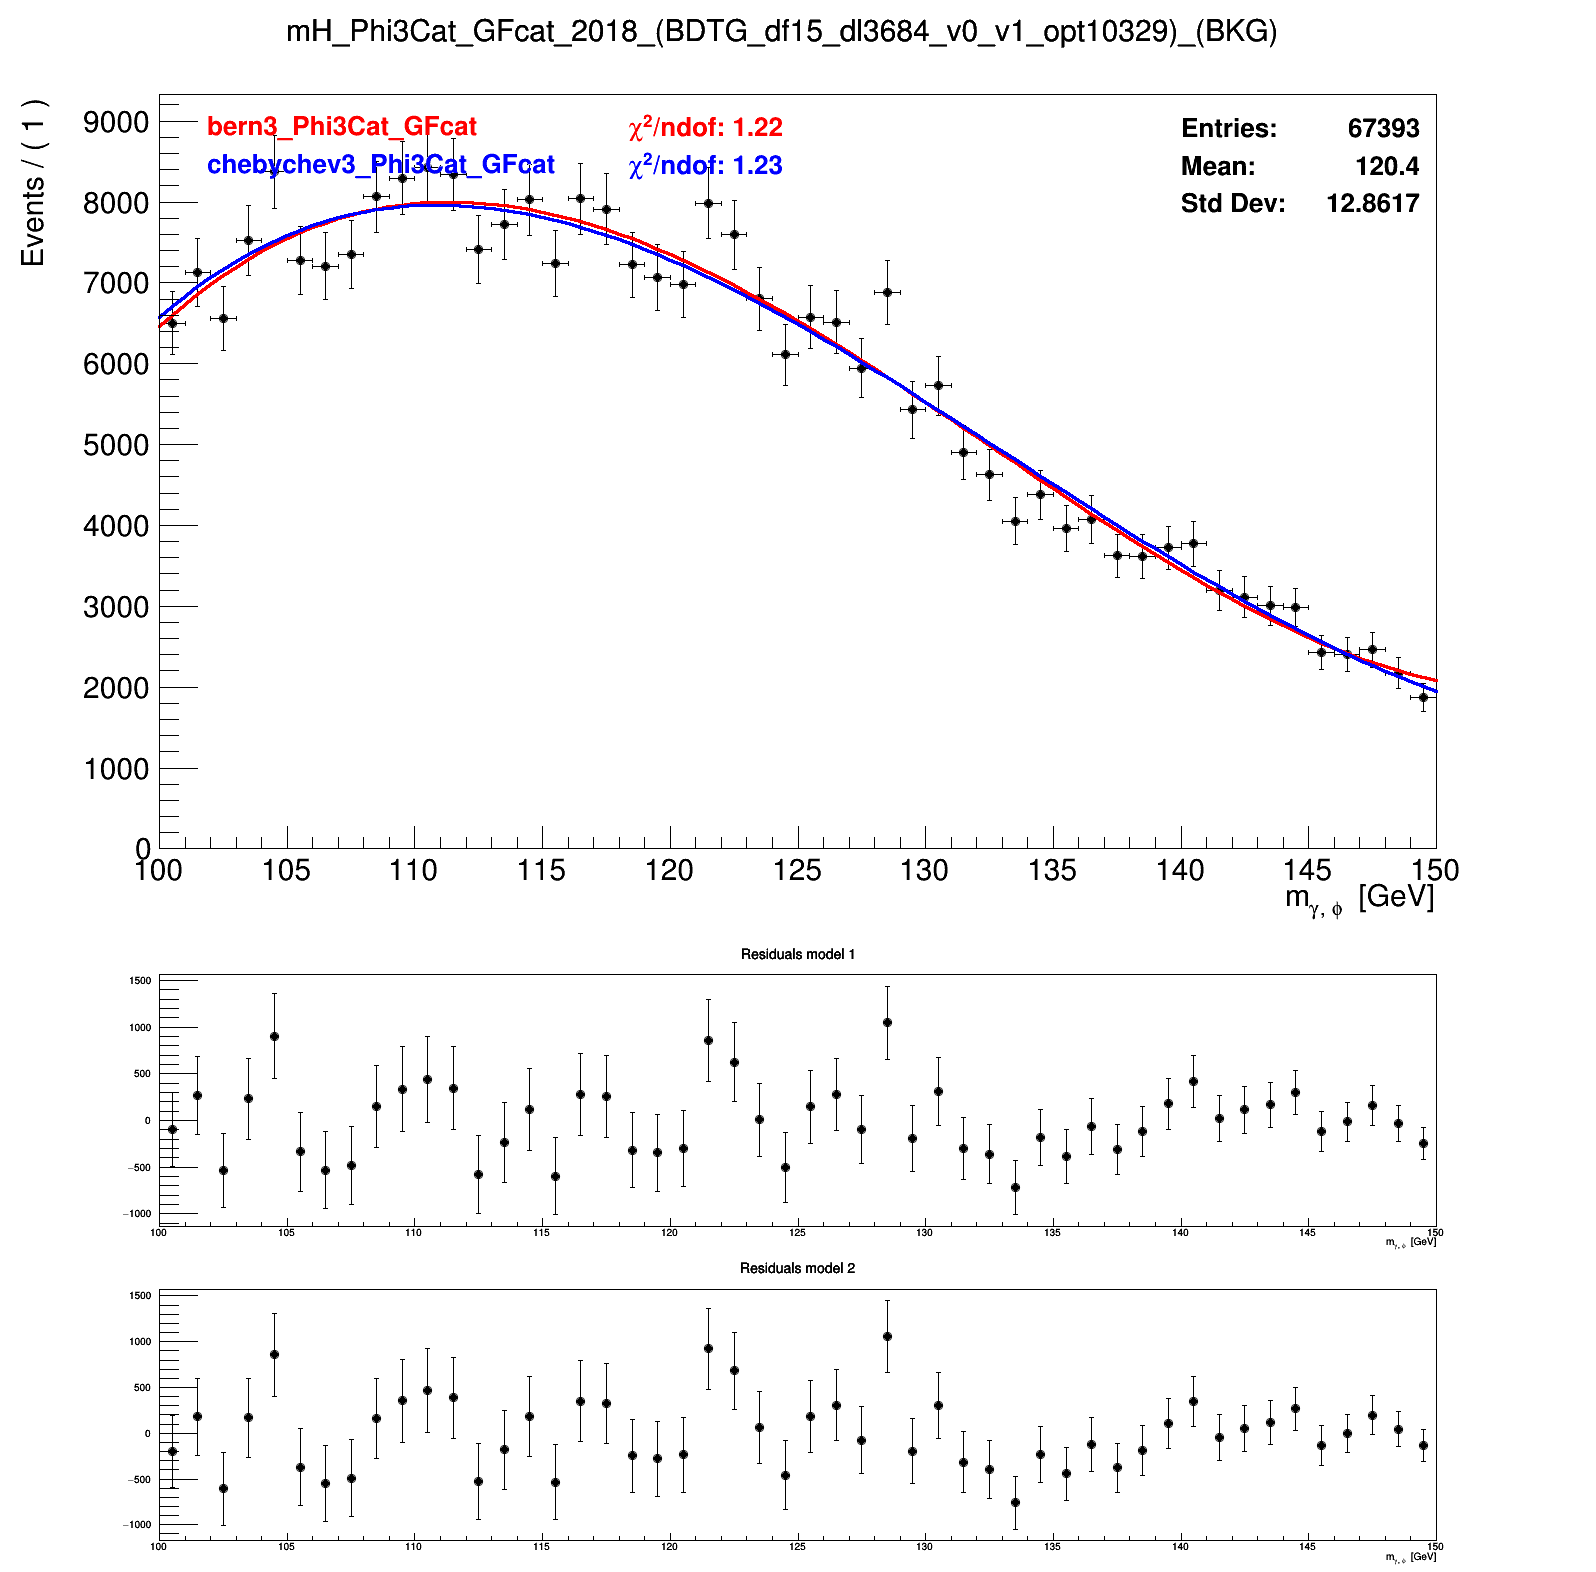
\includegraphics[width=0.45\mylength]{resources/plots/Phi3_fit_BKG.png}
        \caption{\footnotesize (b)}
    \end{subfigure}%\begin{subfigure}[t]{0.50\mylength}\baselineskip
    \vskip\baselineskip
    \vspace*{-0.1cm}
    \begin{subfigure}[t]{0.50\mylength}
        \centering
        \includegraphics[width=0.45\mylength]{resources/plots/Omega_fit_SGN.png}
        \caption{\footnotesize (c)}
    \end{subfigure}%
    \begin{subfigure}[t]{0.50\mylength}
        \centering
        \includegraphics[width=0.45\mylength]{resources/plots/Omega_fit_BKG.png}
        \caption{\footnotesize (d)}
    \end{subfigure}%\begin{subfigure}[t]{0.50\mylength}\baselineskip
\caption{Signal and background fits for the Higgs boson invariant mass for the $\phi$ and $\omega$ decay channels. (a) signal for $\phi$, (b) background for $\phi$, (c) signal for $\omega$, (d) background for $\omega$.}
\label{fig:sig_bkg_modelling_phi_omega}
    \vspace*{-0.0cm}
\end{figure}

\begin{figure}[!ht]
    \captionsetup[subfigure]{labelformat=empty}
    \vspace*{-0.2cm}
    \centering
    \setlength{\mylength}{\textwidth}
    \begin{subfigure}[t]{0.50\mylength}
        \centering
        \includegraphics[width=0.45\mylength]{resources/plots/D0Star_2body_fit_SGN.png}
        \caption{\footnotesize (a)}
    \end{subfigure}%
    \begin{subfigure}[t]{0.50\mylength}
        \centering
        \includegraphics[width=0.45\mylength]{resources/plots/D0Star_2body_fit_BKG.png}
        \caption{\footnotesize (b)}
    \end{subfigure}%\begin{subfigure}[t]{0.50\mylength}\baselineskip
    \vskip\baselineskip
    \vspace*{-0.1cm}
    \begin{subfigure}[t]{0.50\mylength}
        \centering
        \includegraphics[width=0.45\mylength]{resources/plots/D0Star_3body_fit_SGN.png}
        \caption{\footnotesize (c)}
    \end{subfigure}%
    \begin{subfigure}[t]{0.50\mylength}
        \centering
        \includegraphics[width=0.45\mylength]{resources/plots/D0Star_3body_fit_BKG.png}
        \caption{\footnotesize (d)}
    \end{subfigure}%\begin{subfigure}[t]{0.50\mylength}\baselineskip
\caption{Signal and background fits for the Higgs boson invariant mass for the $D^{*0}$ meson in both the 2-body and 3-body decay channels. (a) signal for $D^{*0}$ 2-body, (b) background for $D^{*0}$ 2-body, (c) signal for $D^{*0}$ 3-body, (d) background for $D^{*0}$ 3-body.}
\label{fig:sig_bkg_modelling_d0star}
    \vspace*{-0.0cm}
\end{figure}

\section{Estimated results}\label{sec:results}

The modified frequentist construction CL$_\text{s}$ \cite{Read:2002hq, Junk:1999kv} is used with the asymptotic approximation \cite{Cowan:2010js} to compute 95\% confidence level (CL) upper limits on the branching fractions. For this computation, the Combine tool is employed with the \verb+AsymptoticLimits+ method \cite{CMS:Combine}.

The upper limit is computed by performing a statistical test. Two hypotheses are defined: the null hypothesis $H_0$ describes the model with signal plus background, while the alternative hypothesis $H_1$ represents the background-only hypothesis. Maximum-likelihood fits to the photon-meson invariant mass of the signal plus background MC (or to the data, after unblinding) are done for both hypotheses. The upper limit is then defined as the value of the branching fraction at which we can reject the alternative hypothesis with a $p$-value of 0.05, i.e., at the 95\% CL. The shape of the signal model is determined beforehand, as explained in Section \ref{sec:modelling}, and in this new combined fit, only the normalization constant is allowed to vary. Intuitively, the value of the limit is related to the area under the fitted curves, making it approximately proportional to $\sqrt{S+B}/S$, where $S$ and $B$ are the areas under the signal and background modelled curves, respectively. Additional information can be found in Ref. \cite{Cowan:2010js}.

\todo{How is the limit computed when using the real data for the background estimation with the sidebands?}

Table \ref{tab:results} reports the expected upper limits on the branching ratios.
\begin{table}[!ht]
    \centering
    \begin{tabular}{|l|C{3cm}|C{3cm}|c|}
        \hline
        \multicolumn{1}{|c|}{\cellcolor{lightgray}Decay channel} & \cellcolor{lightgray} Measured $\mathcal{B}$ & \cellcolor{lightgray} ATLAS $\mathcal{B}$ & \cellcolor{lightgray} SM $\mathcal{B}$ \\ \hline
        $\text{H}\decaysto \phi\gamma$          &.\r$x.xx \times 10^{-3}$ &$4.8 \times 10^{-4}$     & $(2.31 \pm 0.11)\times 10^{-6}$  \\
        $\text{H}\decaysto \omega\gamma$        &.\r$x.xx \times 10^{-3}$ &$1.5 \times 10^{-4}$     & $(1.48 \pm 0.08)\times 10^{-6}$  \\
        $\text{H}\decaysto D^{*0}\gamma$ 2-body &.\r$x.xx \times 10^{-3}$ &\multirow{2}{*}{-}       &\multirow{2}{*}{-}  \\
        $\text{H}\decaysto D^{*0}\gamma$ 3-body &.\r$x.xx \times 10^{-3}$ &                         &  \\
        \hline
    \end{tabular}
    \caption{The expected upper limit on the branching fractions for the four studied decay channels is shown in the first column. The second column presents the corresponding upper limits measured by the ATLAS collaboration, when available \cite{ATLAS:2017gko, ATLAS:2023alf}. The third column displays the Standard Model predictions of the branching fractions, when available \cite{Konig:2015qat}.}
    \label{tab:results}
\end{table}

\todo{Comment results}

\section{Future potential improvements}\label{sec:future_improvements}

This analysis provides an initial estimation of the upper limits on the branching ratios of the selected Higgs boson rare decays. Before unblinding and obtaining actual measurements, several improvements, corrections, and cross-checks are necessary. This section will briefly address some of these, although the list is is not exhaustive.
\vspace*{-6pt}
\begin{myitemlist}
    \item[Multivariate analysis signal/background distriminant:] The most important discriminating variable between signal and background processes in this search is the photon-meson invariant mass, which forms a sharp peak around 125 GeV for the signal, as opposed to the background in which it decreases monotonically within the same mass range. Nonetheless, additional kinematic variables can enhance the signal-to-background separation.
    
    To improve the sensitivity, a multivariate discriminant (using BDTs, for example) can be constructed, taking as input several variables that capture the distinct kinematic characteristics of both the signal and the background. To better isolate the Higgs boson signal from the SM background, MVA discriminants should be individually trained for each decay mode.

    These MVA discriminants have shown to reduce the limits by around 44\% - 49\% in similar analyses, like the one the PPC grop is conducting.

    \todo{
        ARE THESE CORRECTIONS ALREADY IMPLEMENTED IN MY ANALYSIS?

    \item[Data - MC corrections:] Simulated signal and background samples should be corrected for various effects through reweighting procedures. This is relevant because the signal is used in the final fit estimation, while the background MC can be used for the training of the MVA discriminant earlier mentioned. These might include:
    \begin{itemize}
        \item {\bf Pileup reweighting:} Pileup conditions in the simulated samples are not identical to the ones observed measured in data, and a reweighting should be applied to remove the difference.
        \item {\bf Photon scale and resolution:} Photon energy scale and resolution corrections should be propagated to the photons. The photon energy scale in data and the resolution in simulation can be evaluated using the $Z^{0}\decaysto ee$ process, like in similar analysis.
        \item {\bf Meson reconstruction:} The track reconstruction efficiency should be applied to the MC events to account for effects associated with the modelling of the tracker material and track reconstruction algorithms.
        \item {\bf Trigger scale factors:} Triggers are applied in the MC selection, so trigger scale factors should be applied to simulation to restore the good data - MC agreement. 
    \end{itemize}
    }

    \item[Bias study in background polynomials:] \todo{Explain}
    \item[Additional Higgs boson production modes:] \todo{Explain}
    \item[Systematics:] \todo{Explain}
\end{myitemlist}

\todo{Add more things?}

